\documentclass{beamer}

%% Packages
\usepackage{graphicx}
\usepackage{amsmath, esint}
\usepackage{ragged2e}
\usepackage{tikz}
\usepackage{listings}
\usepackage{algorithm}
\usepackage{algorithmic}
\usepackage{tabularx}
\usepackage{xcolor} 
\usepackage{amssymb}

%% Packages definitions...
\usetikzlibrary{arrows,shapes}
\lstset{escapeinside={@(}{)@}}
\newcolumntype{Y}{>{\centering\arraybackslash}X}
\definecolor{LightGray}{gray}{0.975}

%% SQL Join symbols...
\def\ojoin{\setbox0=\hbox{$\bowtie$}%
  \rule[-.02ex]{.25em}{.4pt}\llap{\rule[\ht0]{.25em}{.4pt}}}
\def\leftouterjoin{\mathbin{\ojoin\mkern-5.8mu\bowtie}}
\def\rightouterjoin{\mathbin{\bowtie\mkern-5.8mu\ojoin}}
\def\fullouterjoin{\mathbin{\ojoin\mkern-5.8mu\bowtie\mkern-5.8mu\ojoin}}

%% Theme...
\usefonttheme{serif}

\title[Chapter 7]{Database System Concepts, $7^{th}$ Edition \\ Chapter 7: Relational Database Design}
\author{Silberschatz, Korth and Sudarshan}
\date{\today}

%% Remove navigation symbols...
\setbeamertemplate{navigation symbols}{}

%% Footer...
\defbeamertemplate*{footline}{shadow theme}{
    \leavevmode
    \hbox{
        \begin{beamercolorbox}[
                wd =        0.33\paperwidth,
                ht =        2.5ex,
                dp =        1.125ex,
                leftskip =  0.3cm plus1fil,
                rightskip = 0.3cm
            ]{author in head/foot}
            \flushleft DBS
        \end{beamercolorbox}
        \begin{beamercolorbox}[
                wd =        0.33\paperwidth,
                ht =        2.5ex,
                dp =        1.125ex,
                leftskip =  0.3cm plus1fil,
                rightskip = 0.3cm
            ]{author in head/foot}
            \insertshorttitle
        \end{beamercolorbox}
        \begin{beamercolorbox}[
                wd =        0.33\paperwidth,
                ht =        2.5ex,
                dp =        1.125ex,
                leftskip =  0.3cm plus1fil,
                rightskip = 0.3cm
            ]{title in head/foot}
            \hfill \insertframenumber\,/\,\inserttotalframenumber%
        \end{beamercolorbox}
    }
}

%% Agenda...
\AtBeginSection[]
{
     \begin{frame}<beamer>
     \frametitle{Plan}
     \tableofcontents[currentsection]
     \end{frame}
}

%% Align to right...
\newcommand{\toRight}[1]{
    \begin{FlushRight}
        {\tiny #1}
    \end{FlushRight}
}

%%% Let's start %%%
\begin{document}

\frame{\titlepage}

\begin{frame}{Database System Concepts}
    \centering
    
\includegraphics[width=0.5\textwidth]{figures/book_cover.jpg} \\
    \vspace{5mm}
    {
        \tiny
        Content has been extracted from \textit{Database System Concepts}, Seventh Edition, by Silberschatz, Korth and Sudarshan. Mc Graw Hill Education. 2019.\\
        Visit \url{https://db-book.com/}.\\
    }
\end{frame}

\section{Features of Good Relational Design}

\begin{frame}{Features of Good Relational Designs}
    \centering
    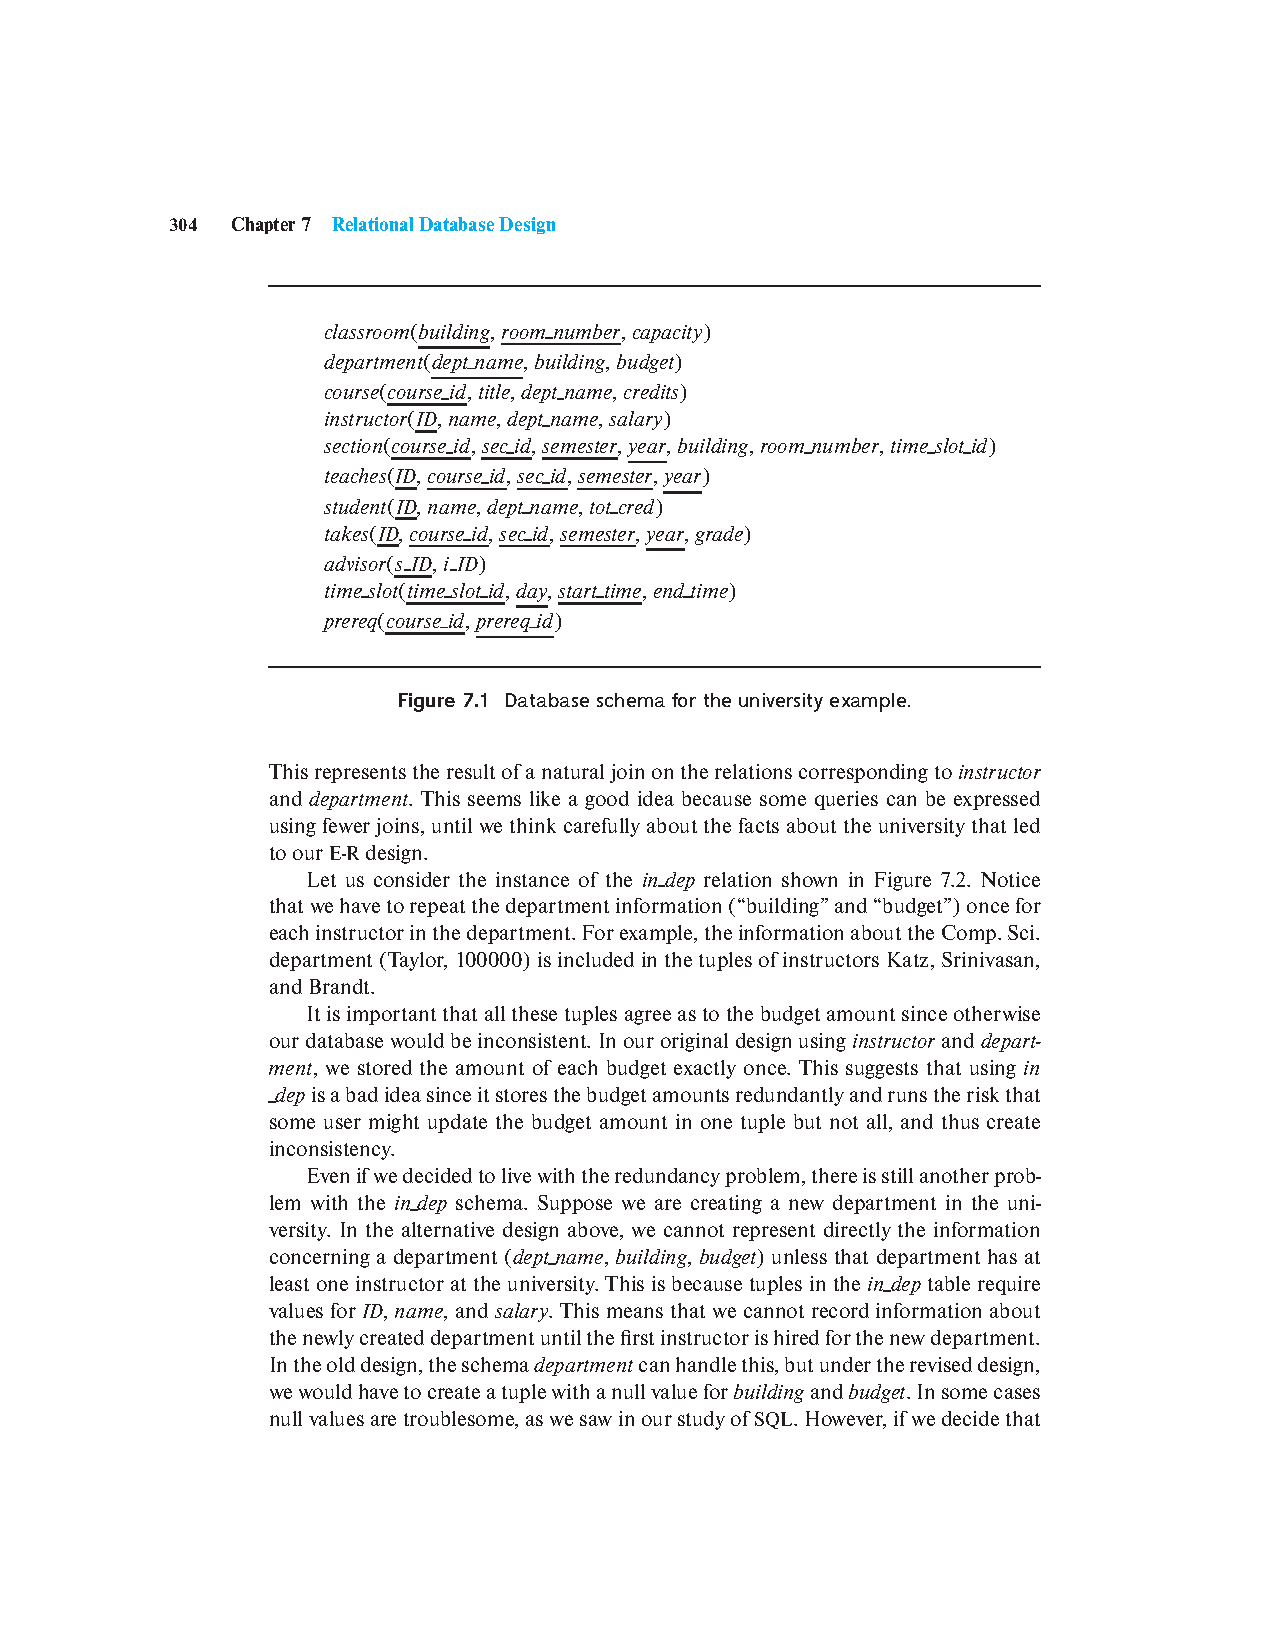
\includegraphics[width=\textwidth, trim={5cm 15.75cm 4cm 4.75cm}, clip]{figures/p304_schema}
\end{frame}

\begin{frame}{Features of Good Relational Designs}
    \begin{itemize}
        \item Suppose we combine \textit{instructor} and \textit{department} into \textit{in\_dep}, which represents the natural join on the relations \textit{instructor} and \textit{department}.
            \begin{center}
                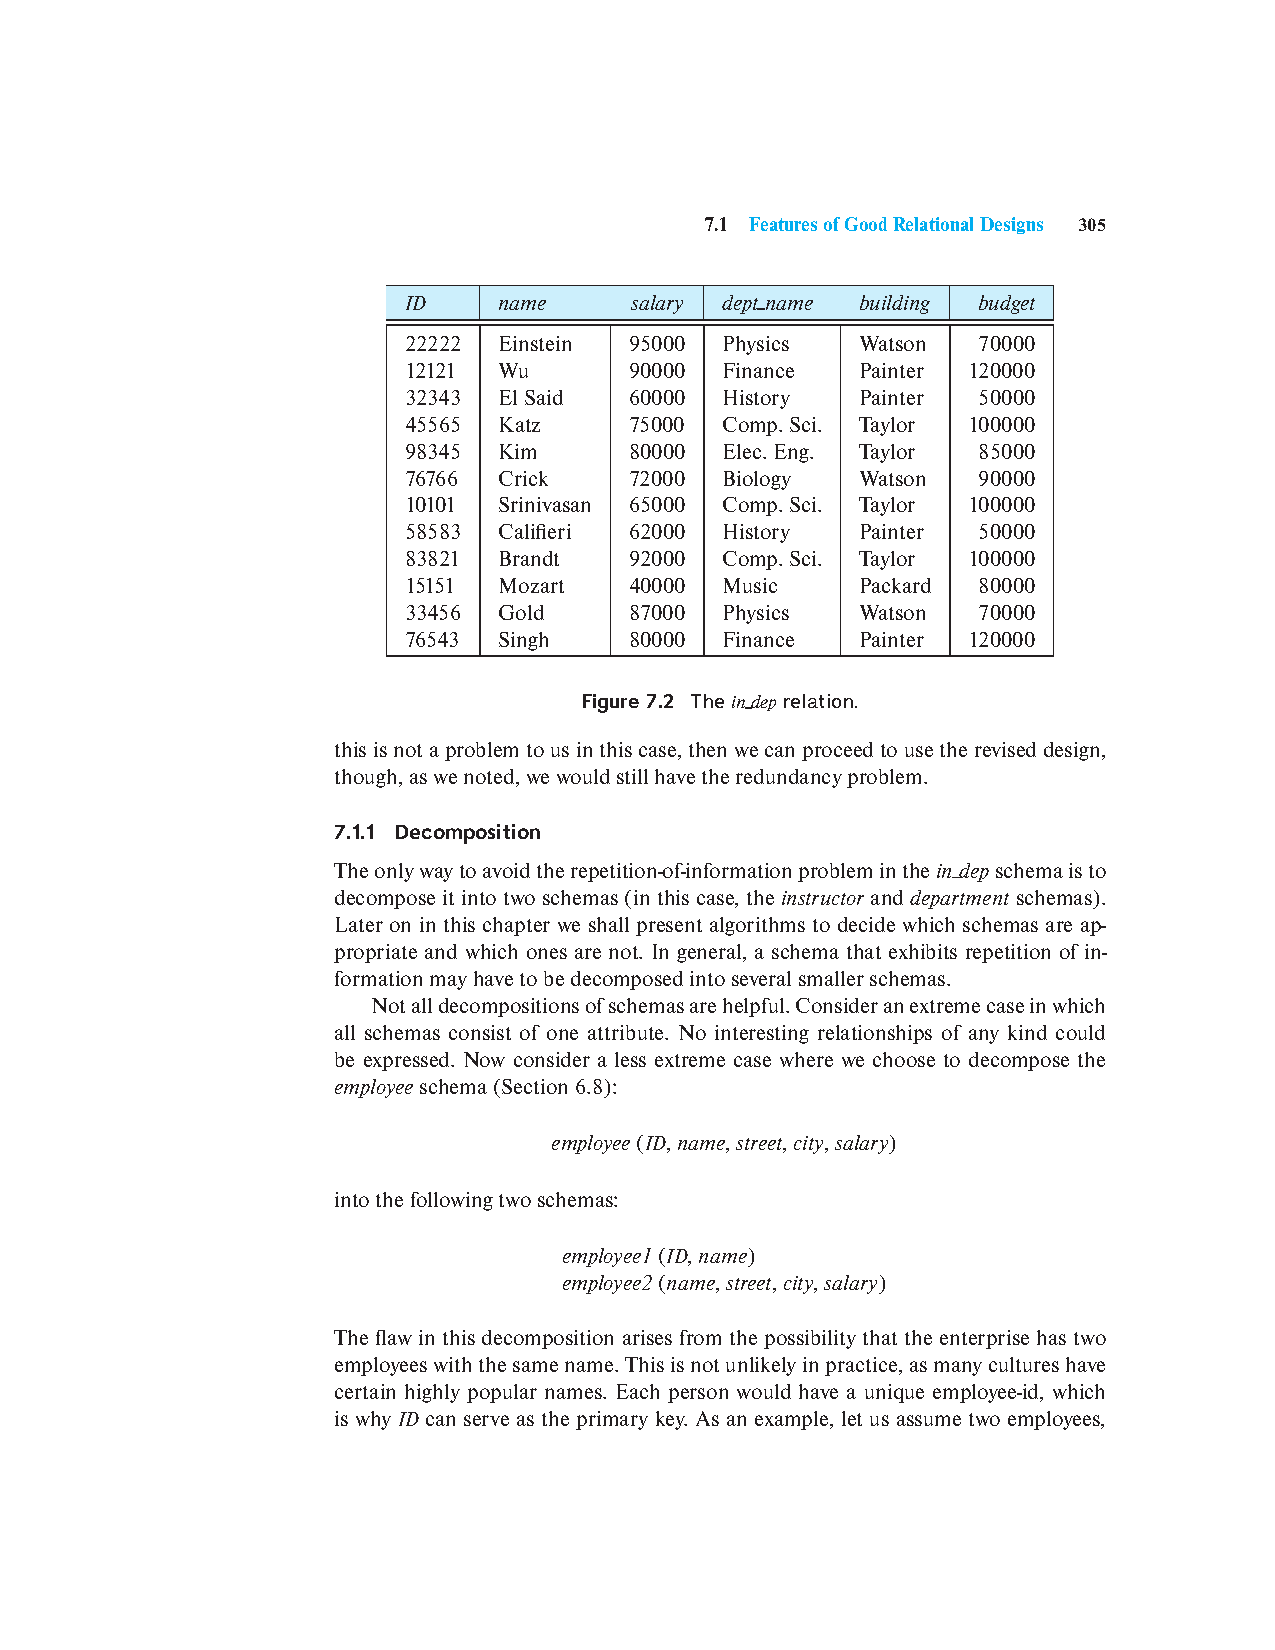
\includegraphics[width=.7\textwidth, trim={5cm 15.75cm 3.75cm 4.75cm}, clip]{figures/p305_in_dep}
            \end{center}
        \item There is repetition of information
        \item Need to use \texttt{\textbf{null}} values (if we add a new department with no instructors)
    \end{itemize}
\end{frame}

\begin{frame}{Decomposition}
    \begin{itemize}
        \item The only way to avoid the repetition-of-information problem in the \textit{in\_dep} schema is to decompose it into two schemas --\textit{instructor} and \textit{department} schemas.
        \item Not all decompositions are good. Suppose we decompose: \\
            \quad \texttt{employee(ID, name, street, city, salary)} \\
            into \\
            \quad \texttt{employee1 (ID, name)} \\
            \quad \texttt{employee2 (name, street, city, salary)} \\
            The problem arises when we have two employees with the same name.
        \item The next slide shows how we lose information --we cannot reconstruct the original employee relation-- and so, this is a \textbf{lossy decomposition}.
    \end{itemize}
\end{frame}

\begin{frame}{A Lossy Decomposition}
    \centering
    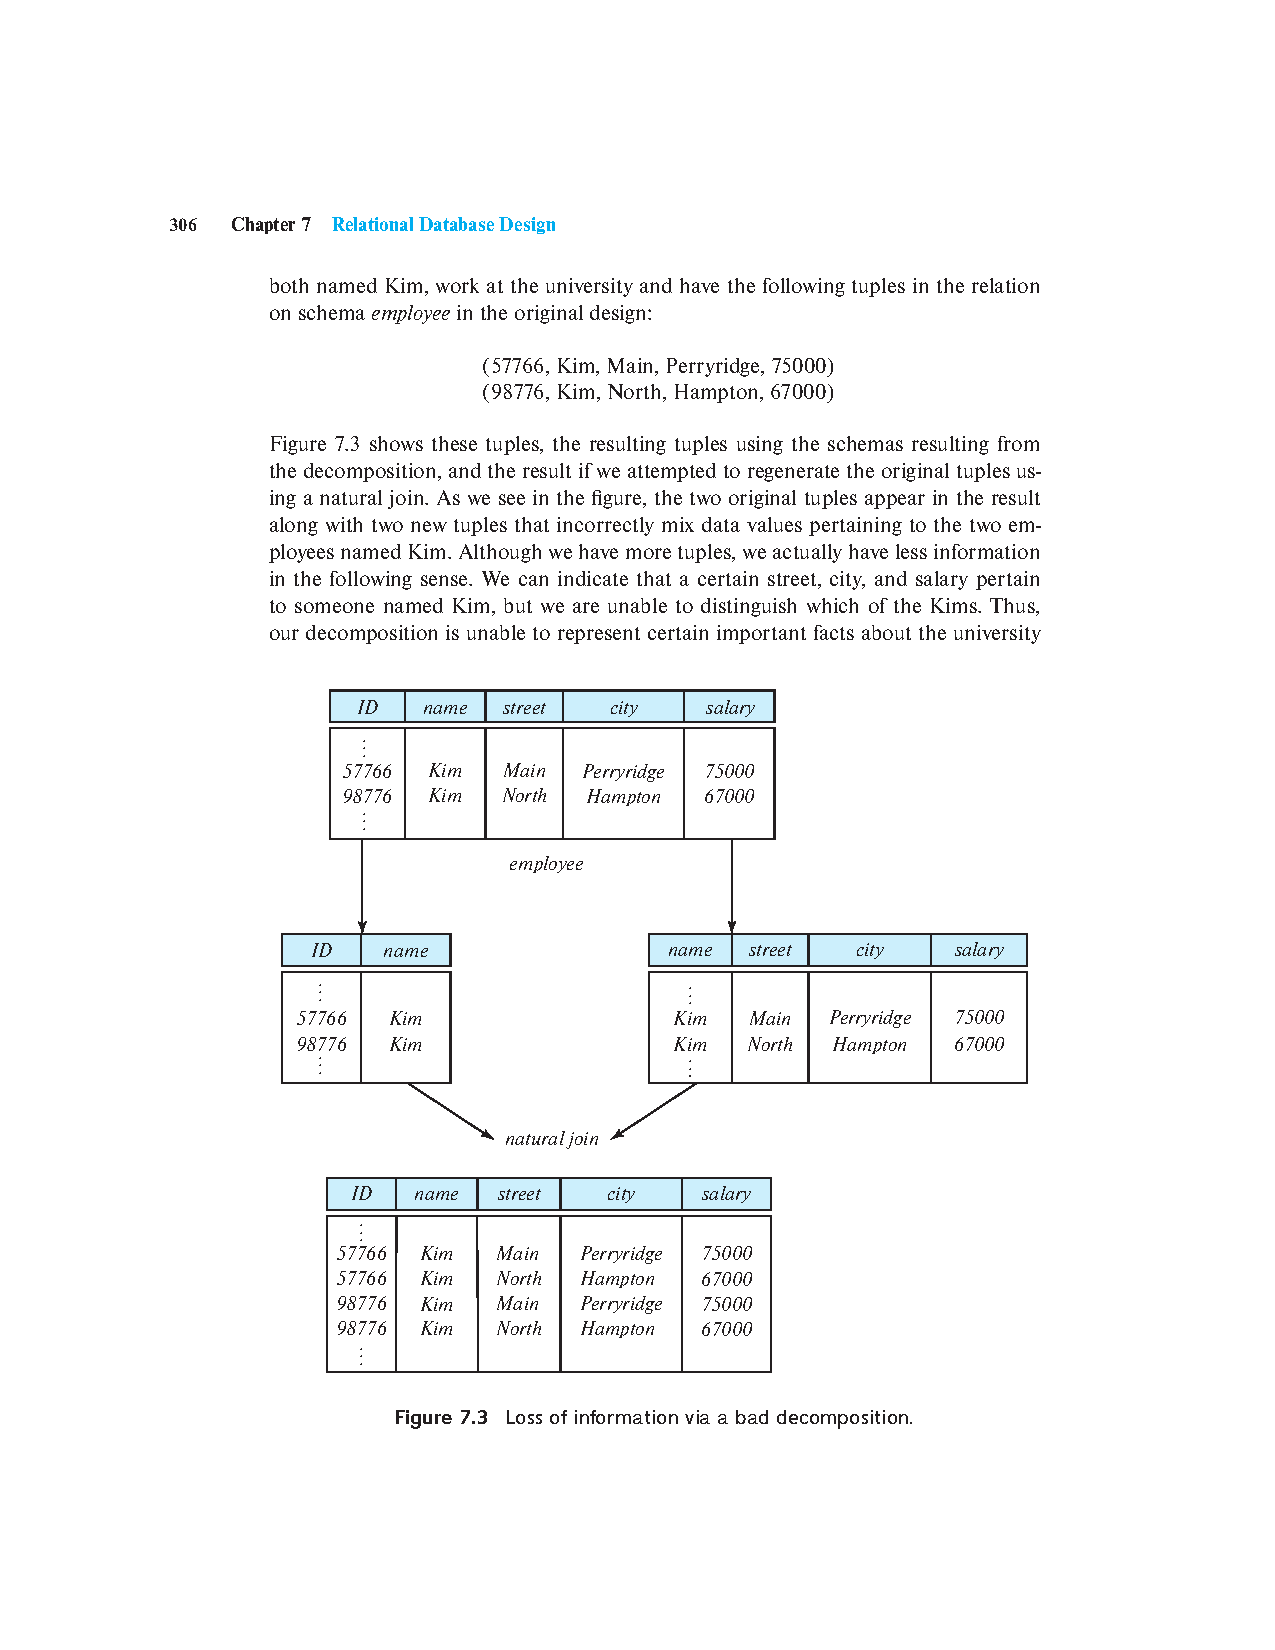
\includegraphics[width=0.85\textwidth, trim={3cm 2cm 4cm 11.25cm}, clip]{figures/p306_loss}
\end{frame}

\begin{frame}{Lossless Decomposition}
    \begin{itemize}
        \item Let $R$ be a relation schema and let $R_1$ and $R_2$ form a decomposition of $R$. That is $R = R_1 \bigcup R_2$.
        \item We say that the decomposition is a \textbf{lossless decomposition} if there is no loss of information by replacing $R$ with the two relation schemas $R_1 \bigcup R_2$.
        \item Formally,
            $$
                \Pi_{R_1}(r) \Join \Pi_{R_2}(r) = r
            $$
        \item And, conversely a decomposition is lossy if
            $$
                r \subset \Pi_{R_1}(r) \Join \Pi_{R_2}(r)
            $$
    \end{itemize}
\end{frame}

\begin{frame}{Example of Lossless Decomposition}
    \begin{itemize}
        \item Decomposition of $R = (A, B, C)$:
            $$
                R_1 = (A, B); R_2 = (B, C)
            $$
    \end{itemize}
    \centering
    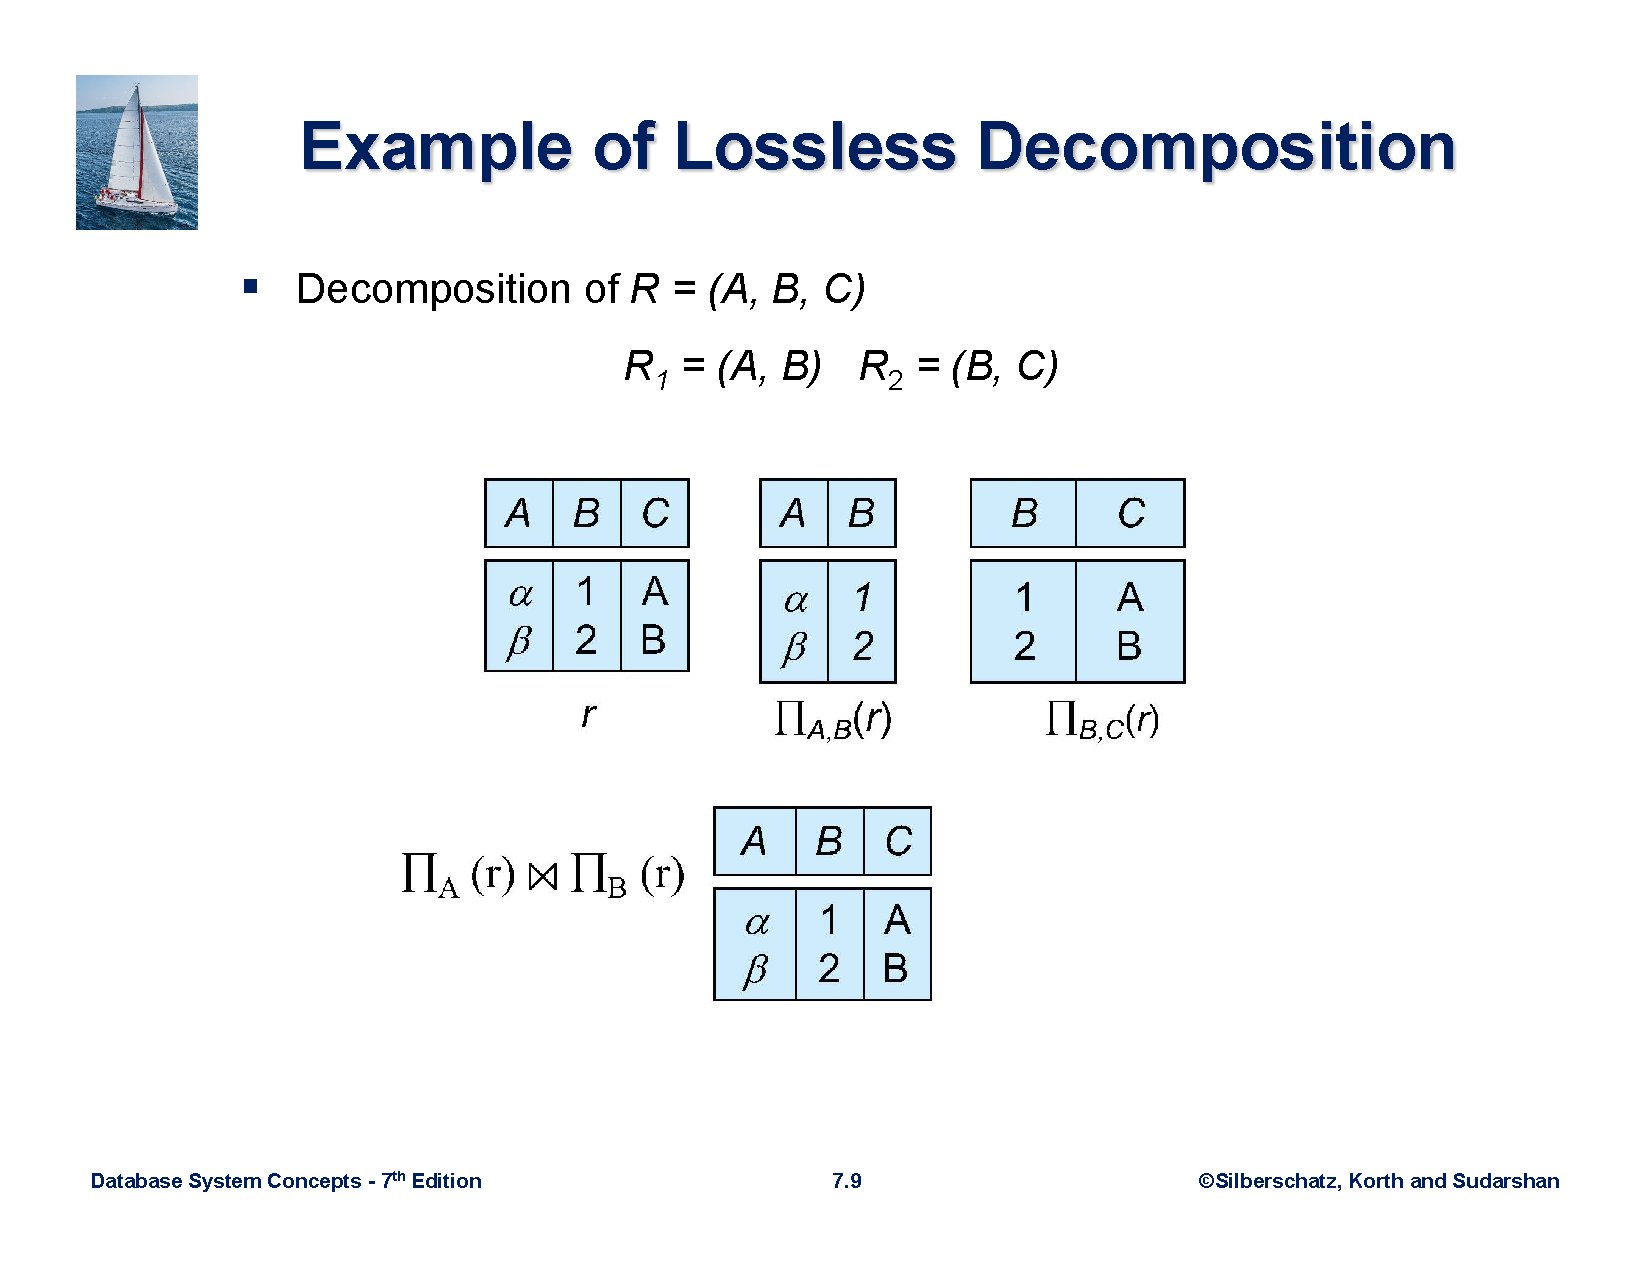
\includegraphics[width=\textwidth, trim={3cm 2cm 3cm 8cm}, clip]{figures/slide7_loss}
\end{frame}

\begin{frame}{Normalization Theory}
    \begin{itemize}
        \item Decide whether a particular relation $R$ is in ``good'' form.
        \item In the case that a relation $R$ is not in ``good'' form, decompose it into set of relations $\{R_1, R_2, \cdots, R_n\}$ such that,
        \begin{itemize}
            \item Each relation is in good form.
            \item The decomposition is a lossless decomposition.
        \end{itemize}
        \item Our theory is based on:
        \begin{enumerate}
            \item functional dependencies.
            \item multivalued dependencies.
        \end{enumerate}
    \end{itemize}
\end{frame}

\section{Functional Dependencies}

\begin{frame}{Functional Dependencies}
    \begin{itemize}
        \item There are usually a variety of constraints (rules) on the data in the real world.
        \item For example, some of the constraints that are expected to hold in a university database are:
        \begin{itemize}
            \item Students and instructors are uniquely identified by their ID.
            \item Each student and instructor has only one name.
            \item Each instructor and student is (primarily) associated with only one department.
            \item Each department has only one value for its budget, and only one associated building.
        \end{itemize}
    \end{itemize}
\end{frame}

\begin{frame}{Functional Dependencies (Cont.)}
    \begin{itemize}
        \item An instance of a relation that satisfies all such real-world constraints is called a \textbf{legal instance} of the relation.
        \item A legal instance of a database is one where all the relation instances are legal instances.
        \item Require that the value for a certain set of attributes determines uniquely the value for another set of attributes.
        \item A functional dependency is a generalization of the notion of a key.
    \end{itemize}
\end{frame}

\begin{frame}{Functional Dependencies Definition}
    \begin{itemize}
        \footnotesize
        \item Let $R$ be a relation schema
            \begin{equation*}
                \begin{align*}
                    \alpha \subseteq R \text{ and } \beta \subseteq R
                \end{align*}
            \end{equation*}
        \item The \textbf{functional dependency}
            $$
                \alpha \rightarrow \beta
            $$
            \textbf{holds on} $R$ if and only if for any legal relations $r(R)$, whenever any two tuples $t_1$ and $t_2$ of $r$ agree on the attributes $\alpha$, they also agree on the attributes $\beta$. That is,
            $$
                t_1[\alpha] = t_2[\alpha] \Rightarrow t_1[\beta] = t_2 [\beta]
            $$
        \item Example: Consider $r(A,B)$ with the following instance of $r$: \\
            \centering
            \begin{tabular}{|c|c|}
                \hline
                \textbf{A} & \textbf{B} \\ \hline
                1 & 4 \\ \hline
                1 & 5 \\ \hline
                3 & 7 \\ \hline
            \end{tabular}
        \item On this instance, $B \rightarrow A$ hold; $A \rightarrow B$ does \textbf{NOT} hold,
    \end{itemize}
\end{frame}

\begin{frame}{Closure of a Set of Functional Dependencies}
    \begin{itemize}
        \item Given a set $F$ set of functional dependencies, there are certain other functional dependencies that are logically implied by $F$.
        \begin{itemize}
            \item If $A \rightarrow B$ and $B \rightarrow C$, then we can infer that $A \rightarrow C$.
        \end{itemize}
        \item The set of \textbf{all} functional dependencies logically implied by $F$ is the \textbf{closure} of $F$.
        \item We denote the closure of $F$ by $F^+$.
    \end{itemize}
\end{frame}

\section{Decomposition Using Functional Dependencies}

\begin{frame}{Keys and Functional Dependencies}
    \begin{itemize}
        \item $K$ is a superkey for relation schema $R$ if and only if $K \rightarrow R$.
        \item $K$ is a primary key for $R$ if and only if:
        \begin{itemize}
            \item $K \rightarrow R$, and
            \item for no $\alpha \subset K, \alpha \rightarrow R$
        \end{itemize}
        \item Functional dependencies allow us to express constraints that cannot be expressed using superkeys. Consider the schema:
            \begin{center}
                \texttt{\footnotesize in\_dep(ID, name, salary, dept\_name, building, budget)}.
            \end{center}
        We expect these functional dependencies to hold:
            \begin{equation*}
                \begin{align*}
                    dept\_name \rightarrow& building \\
                    ID \rightarrow& building
                \end{align*}
            \end{equation*}
        but would not expect the following to hold:
            \begin{equation*}
                \begin{align*}
                    dept\_name \rightarrow& salary
                \end{align*}
            \end{equation*}
    \end{itemize}
\end{frame}

\begin{frame}{Use of Functional Dependencies}
    \begin{itemize}
        \item We use functional dependencies to:
        \begin{itemize}
            \item To test relations to see if they are legal under a given set of functional dependencies.
            \begin{itemize}
                \item If a relation $r$ is legal under a set $F$ of functional dependencies, we say that $r$ \textbf{satisfies} $F$.
            \end{itemize}
            \item To specify constraints on the set of legal relations.
            \begin{itemize}
                \item We say that $F$ \textbf{holds on} $R$ if all legal relations on $R$ satisfy the set of functional dependencies $F$.
            \end{itemize}
        \end{itemize}
        \item Note: A specific instance of a relation schema may satisfy a functional dependency even if the functional dependency does not hold on all legal instances.
        \begin{itemize}
            \item For example, a specific instance of \textit{instructor} may, by chance, satisfy
            $$
                name \rightarrow ID.
            $$
        \end{itemize}
    \end{itemize}
\end{frame}

\begin{frame}{Trivial Functional Dependencies}
    \begin{itemize}
        \item A functional dependency is \textbf{trivial} if it is satisfied by all instances of a relation.
        \begin{itemize}
            \item Example:
            \begin{itemize}
                \item $ID, name \rightarrow ID$
                \item $name \rightarrow name$
            \end{itemize}
            \item In general, $\alpha \rightarrow \beta$ is trivial if $\beta \subseteq \alpha$.
        \end{itemize}
    \end{itemize}
\end{frame}

\begin{frame}{Lossless Decomposition}
    \begin{itemize}
        \item We can use functional dependencies to show when certain decomposition are lossless.
        \item For the case of $R = (R_1, R_2)$, we require that for all possible relations $r$ on schema $R$
            $$
                r = \Pi_{R_1}(r) \Join \Pi_{R_2}(r)
            $$
        \item A decomposition of $R$ into $R_1$ and $R_2$ is lossless decomposition if at least one of the following dependencies is in $F^+$:
        \begin{equation*}
            \begin{align*}
                R_1 \bigcap R_2 \rightarrow& R_1 \\
                R_1 \bigcap R_2 \rightarrow& R_2
            \end{align*}
        \end{equation*}
        \item The above functional dependencies are a sufficient condition for lossless join decomposition; the dependencies are a necessary condition only if all constraints are functional dependencies.
    \end{itemize}
\end{frame}

\begin{frame}{Example\footnote{Note: $B \rightarrow BC$ is a shorthand notation for $B \rightarrow \{B, C\}$.}}
    \begin{itemize}
        \item $R = (A, B, C)$
            \begin{equation*}
                \begin{align*}
                    F = \{  A \rightarrow& B \\
                            B \rightarrow& C\}
                \end{align*}
            \end{equation*}

        \item $R_1 = (A, B)$; $R_2 = (B, C)$ \\
            \text{Lossless decomposition:} \\
            $R_1 \bigcap R_2 = \{B\}$  and $B \rightarrow BC$ holds.
        \item $R_1 = (A, B)$; $R_2 = (A, C)$ \\
            \text{Lossless decomposition:} \\
            $R_1 \bigcap R_2 = \{A\}$  and $A \rightarrow AC$ holds.
    \end{itemize}
\end{frame}

\begin{frame}{Dependency Preservation}
    \begin{itemize}
        \item Testing functional dependency constraints each time the database is updated can be costly,
        \item It is useful to design the database in a way that constraints can be tested efficiently.
        \item If testing a functional dependency can be done by considering just one relation, then the cost of testing this constraint is low.
        \item When decomposing a relation it is possible that it is no longer possible to do the testing without having to perform a Cartesian Produced.
        \item A decomposition that makes it computationally hard to enforce functional dependency is said to be NOT \textbf{dependency preserving}.
    \end{itemize}
\end{frame}

\begin{frame}{Dependency Preservation Example}
    \begin{itemize}
        \item Consider a schema:
            \begin{center}
                \texttt{dept\_advisor(s\_ID, i\_ID, department\_name)}
            \end{center}
        \item With function dependencies:
            \begin{center}
                $i\_ID \rightarrow dept\_name$ \\
                $s\_ID, dept\_name \rightarrow i\_ID$
            \end{center}
        \item In the above design we are forced to repeat the department name once for each time an instructor participates in a \textit{dept\_advisor} relationship.
        \item To fix this, we need to decompose \textit{dept\_advisor}.
        \item Any decomposition will not include all the attributes in:
            \begin{center}
                $s\_ID, dept\_name \rightarrow i\_ID$
            \end{center}
        \item Thus, the composition NOT be dependency preserving.
    \end{itemize}
\end{frame}

\section{Normal Forms}

\begin{frame}{Boyce-Codd Normal Form}
    \begin{itemize}
        \item A relation schema $R$ is in BCNF with respect to a set $F$ of functional dependencies if for all functional dependencies in $F^+$ of the form:
        $$
            \alpha \rightarrow \beta
        $$
        where $\alpha \subseteq R$ and $\beta \subseteq R$, at least one of the following holds:
        \begin{itemize}
            \item $\alpha \rightarrow \beta$ is trivial (i.e., $\beta \subseteq \alpha$)
            \item $\alpha$ is a superkey for $R$.
        \end{itemize}
    \end{itemize}
\end{frame}

\begin{frame}{Boyce-Codd Normal Form (Cont.)}
    \begin{itemize}
        \item Example schema that is not in BCNF: \\
            \begin{center}
                \texttt{\footnotesize in\_dep (ID, name, salary, dept\_name, building, budget)}
            \end{center}
        because :
        \begin{itemize}
            \item $dept\_name \rightarrow building, budget$
            \begin{itemize}
                \item holds on \texttt{in\_dep}
                \item but...
            \end{itemize}
            \item \textit{dept\_name} is not a superkey.
        \end{itemize}
        \item When decompose \texttt{in\_dept} into \texttt{instructor} and \texttt{department}:
        \begin{itemize}
            \item \texttt{instructor} is in BCNF.
            \item \texttt{department} is in BCNF.
        \end{itemize}
    \end{itemize}
\end{frame}

\begin{frame}{Decomposing a Schema into BCNF}
    \begin{itemize}
        \item Let $R$ be a schema that is not in BCNF. Let $\alpha \rightarrow \beta$ be the Fuctional Dependency that causes a violation of BCNF.
        \item We decompose $R$ into:
            \begin{itemize}
                \item $(\alpha \bigcup \beta)$
                \item $(R - (\beta - \alpha))$
            \end{itemize}
        \item In our example of \texttt{in\_dep},
            \begin{itemize}
                \item $\alpha = dept\_name$
                \item $\beta = building, budget$
            \end{itemize}
        and \texttt{in\_dep} is replaced by
            \begin{itemize}
                \item $(\alpha \bigcup \beta) = (dept\_name, building, budget)$
                \item $(R - (\beta - \alpha)) = (ID, name, salary, dept\_name)$
            \end{itemize}
    \end{itemize}
\end{frame}

\begin{frame}{BCNF and Dependency Preservation}
    \begin{itemize}
        \item It is not always possible to achieve both BCNF and dependency preservation.
        \item Consider a schema:
            \begin{center}
                \texttt{dept\_advisor(s\_ID, i\_ID, department\_name)}
            \end{center}
        \item With function dependencies:\\
            \begin{tabular}{r l}
                $i\_ID \rightarrow$ & $dept\_name$ \\
                $s\_ID, dept\_name \rightarrow$ & $i\_ID$
            \end{tabular}
        \item \texttt{dept\_advisor} is not in BCNF:
            \begin{itemize}
                \item \textit{i\_ID} is not a superkey.
            \end{itemize}
        \item Any decomposition of \texttt{dept\_advisor} will not include all the attributes in: \\
            \begin{tabular}{r l}
                $s\_ID, dept\_name \rightarrow$ & $i\_ID$
            \end{tabular}
        \item Thus, the composition is NOT be dependency preserving.
    \end{itemize}
\end{frame}

\begin{frame}{Third Normal Form}
    \begin{itemize}
        \item A relation schema R is in \textbf{third normal form (3NF)} if for all:
            \begin{center}
                $\alpha \rightarrow \beta$ in $F^+$
            \end{center}
        at least one of the following holds:
            \begin{itemize}
                \item $\alpha \rightarrow \beta$ is trivial (i.e., $\beta \in \alpha$).
                \item $\alpha$ is a superkey for $R$.
                \item Each attribute $A$ in $\beta - \alpha$ is contained in a candidate key\footnote{NOTE: each attribute may be in a different candidate key.} for $R$.
            \end{itemize}
        \item If a relation is in BCNF it is in 3NF (since in BCNF one of the first two conditions above must hold).
        \item Third condition is a minimal relaxation of BCNF to ensure dependency preservation (will see why later).
    \end{itemize}
\end{frame}

\begin{frame}{3NF Example}
    \begin{itemize}
        \item Consider a schema:
            \begin{center}
                \texttt{dept\_advisor(s\_ID, i\_ID, dept\_name)}
            \end{center}
        \item With function dependencies:
            \begin{equation*}
                \begin{align*}
                    i\_ID \rightarrow& dept\_name \\
                    s\_ID, dept\_name \rightarrow& i\_ID
                \end{align*}
            \end{equation*}
        \item Two candidate keys = $\{s\_ID, dept\_name\}$, $\{s\_ID, i\_ID\}$
        \item We have seen before that \texttt{dept\_advisor} is not in BCNF.
        \item R, however, is in 3NF:
            \begin{itemize}
                \item $s\_ID$, $dept\_name$ is a superkey,
                \item $i\_ID \rightarrow dept\_name$ and $i\_ID$ is NOT a superkey, but:
                    \begin{itemize}
                        \item ${dept\_name} - {i\_ID} = {dept\_name}$ and
                        \item $dept\_name$ is contained in a candidate key.
                    \end{itemize}
            \end{itemize}
    \end{itemize}
\end{frame}

\begin{frame}{Redundancy in 3NF}
    \begin{itemize}
        \item Consider the schema $R$ below, which is in 3NF:
            \begin{itemize}
                \item $R = (J, K, L )$,
                \item $F = \{JK \rightarrow L, L \rightarrow K \}$,
                \item And an instance table:
                    \begin{center}
                        \begin{tabular}{| c | c | c |}
                            \hline
                            J     & L     & K     \\
                            \hline
                            $j_1$ & $l_1$ & $k_1$ \\
                            $j_2$ & $l_1$ & $k_1$ \\
                            $j_3$ & $l_1$ & $k_1$ \\
                            \texttt{\textbf{null}} & $l_2$ & $k_2$ \\
                            \hline
                        \end{tabular}
                    \end{center}
            \end{itemize}
        \item What is wrong with the table? \pause
            \begin{itemize}
                \item Repetition of information,
                \item Need to use \texttt{\textbf{null}} values (e.g., to represent the relationship $l_2$, $k_2$ where there is no corresponding value for $J$)
            \end{itemize}
    \end{itemize}
\end{frame}

\begin{frame}{Comparison of BCNF and 3NF}
    \begin{itemize}
        \item Advantages to 3NF over BCNF. It is always possible to obtain a 3NF design without sacrificing losslessness or dependency preservation.
        \item Disadvantages to 3NF.
            \begin{itemize}
                \item We may have to use \texttt{\textbf{null}} values to represent some of the possible meaningful relationships among data items.
                \item There is the problem of repetition of information.
            \end{itemize}
    \end{itemize}
\end{frame}

\begin{frame}{Goals of Normalization}
    \begin{itemize}
        \item Let $R$ be a relation scheme with a set $F$ of functional dependencies.
        \item Decide whether a relation scheme $R$ is in ``good'' form.
        \item In the case that a relation scheme $R$ is not in ``good'' form, decompose it into a set of relation scheme $\{R_1, R_2, \cdots, R_n\}$ such that:
            \begin{itemize}
                \item Each relation scheme is in good form,
                \item The decomposition is a lossless decomposition,
                \item Preferably, the decomposition should be dependency preserving.
            \end{itemize}
    \end{itemize}
\end{frame}

\begin{frame}{How good is BCNF?}
    \begin{itemize}
        \item There are database schemas in BCNF that do not seem to be sufficiently normalized...
        \item Consider a relation:
            \begin{center}
                \texttt{inst\_info(ID, child\_name, phone)}
            \end{center}
        where an instructor may have more than one phone and can have multiple children.
        \item Instance of \texttt{inst\_info}
            \begin{center}
                \begin{tabular}{ c c c}
                    \hline
                    \textbf{ID} & \textbf{child\_name} & \textbf{phone} \\
                    \hline
                    99999 & David   & 512-555-1234 \\
                    99999 & David   & 512-555-4321 \\
                    99999 & William & 512-555-1234 \\
                    99999 & William & 512-555-4321 \\
                    \hline
                \end{tabular}
            \end{center}
    \end{itemize}
\end{frame}

\begin{frame}{How good is BCNF? (Cont.)}
    \begin{itemize}
        \item There are no non-trivial functional dependencies and therefore the relation is in BCNF.
        \item Insertion anomalies -- i.e., if we add a phone 981-992-3443 to 99999, we need to add two tuples:
            \begin{center}
                \begin{tabular}{l}
                    (99999, David, 981-992-3443) \\
                    (99999, William, 981-992-3443)
                \end{tabular}
            \end{center}
    \end{itemize}
\end{frame}

\begin{frame}{Higher Normal Forms}
    \begin{itemize}
        \item It is better to decompose \texttt{inst\_info} into:
            \begin{itemize}
                \item \texttt{inst\_child}
                    \begin{center}
                        \begin{tabular}{r r}
                            \hline
                            \textbf{ID} & \textbf{child\_name} \\
                            \hline
                            99999 & David   \\
                            99999 & William \\
                            \hline
                        \end{tabular}
                    \end{center}
                \item \texttt{inst\_phone}
                    \begin{center}
                        \begin{tabular}{r r}
                            \hline
                            \textbf{ID} & \textbf{phone} \\
                            \hline
                            99999 & 512-555-1234 \\
                            99999 & 512-555-4321 \\
                            \hline
                        \end{tabular}
                    \end{center}
            \end{itemize}
        \item This suggests the need for higher normal forms, such as Fourth Normal Form (4NF), which we shall see later
    \end{itemize}
\end{frame}

\section{Functional Dependency Theory}

\begin{frame}{Functional-Dependency Theory Roadmap}
    \begin{itemize}
        \item We now consider the formal theory that tells us which functional dependencies are implied logically by a given set of functional dependencies.
        \item We then develop algorithms to generate lossless decompositions into BCNF and 3NF.
        \item We then develop algorithms to test if a decomposition is dependency-preserving.
    \end{itemize}
\end{frame}

\begin{frame}{Closure of a Set of Functional Dependencies}
    \begin{itemize}
        \item Given a set F set of functional dependencies, there are certain other functional dependencies that are logically implied by F.
            \begin{itemize}
                \item If $A \rightarrow B$ and $B \rightarrow C$, then we can infer that $A \rightarrow C$
                \item etc.
            \end{itemize}
        \item The set of all functional dependencies logically implied by $F$ is the closure of $F$.
        \item We denote the closure of $F$ by $F^+$.
    \end{itemize}
\end{frame}

\begin{frame}{Closure of a Set of Functional Dependencies}
    \begin{itemize}
        \item We can compute $F^+$, the closure of $F$, by repeatedly applying \textbf{Armstrong's Axioms}:
            \begin{itemize}
                \item \textbf{Reflexive rule}: if $\beta \subseteq \alpha$, then $\alpha \rightarrow \beta$,
                \item \textbf{Augmentation rule}: if $\alpha \rightarrow \beta$, then $\gamma \alpha \rightarrow \gamma \beta$,
                \item \textbf{Transitivity rule}: if $\alpha \rightarrow \beta$, and $\beta \rightarrow \gamma$, then $\alpha \rightarrow \gamma$.
            \end{itemize}
        \item These rules are:
            \begin{itemize}
                \item \textbf{sound} -- generate only functional dependencies that actually hold, and
                \item \textbf{complete} -- generate all functional dependencies that hold.
            \end{itemize}
    \end{itemize}
\end{frame}

\begin{frame}{Example of $F^+$}
    \begin{itemize}
        \item $R = (A, B, C, G, H, I)$
            \begin{equation*}
                \begin{align*}
                    F=\{A \rightarrow& B \\
                        A \rightarrow& C \\
                       CG \rightarrow& H \\
                       CG \rightarrow& I \\
                        B \rightarrow& H\} \\
                \end{align*}
            \end{equation*}
        \item Some members of $F^+$
            \begin{itemize}
                \item $A \rightarrow H$ by transitivity from $A \rightarrow B$ and $B \rightarrow H$.
                \item $AG \rightarrow I$ by augmenting $A \rightarrow C$ with $G$, to get $AG \rightarrow CG$ and then transitivity with $CG \rightarrow I$.
                \item $CG \rightarrow HI$ by augmenting $CG \rightarrow I$ to infer $CG \rightarrow CGI$, and augmenting of $CG \rightarrow H$ to infer $CGI \rightarrow HI$, and then transitivity.
            \end{itemize}
    \end{itemize}
\end{frame}

\begin{frame}{Closure of a Set of Functional Dependencies (Cont.)}
    \begin{itemize}
        \item Additional rules:
            \begin{itemize}
                \item \textbf{Union rule}: If $\alpha \rightarrow \beta$ holds and $\alpha \rightarrow \gamma$ holds, then $\alpha \rightarrow \beta \gamma$ holds.
                \item \textbf{Decomposition rule}: If $\alpha \rightarrow \beta \gamma$ holds, then $\alpha \rightarrow \beta$ holds and $\alpha \rightarrow \gamma$ holds.
                \item \textbf{Pseudotransitivity rule}: If $\alpha \rightarrow \beta$ holds and $\gamma \beta \rightarrow \delta$ holds, then $\alpha \gamma \rightarrow \delta$ holds.
            \end{itemize}
        \item The above rules can be inferred from Armstrong's axioms.
    \end{itemize}
\end{frame}

\begin{frame}{Procedure for Computing $F^+$}
    \begin{itemize}
        \item To compute\footnote{NOTE: We shall see an alternative procedure for this task later.} the closure of a set of functional dependencies $F$:
    \end{itemize}
    \centering
    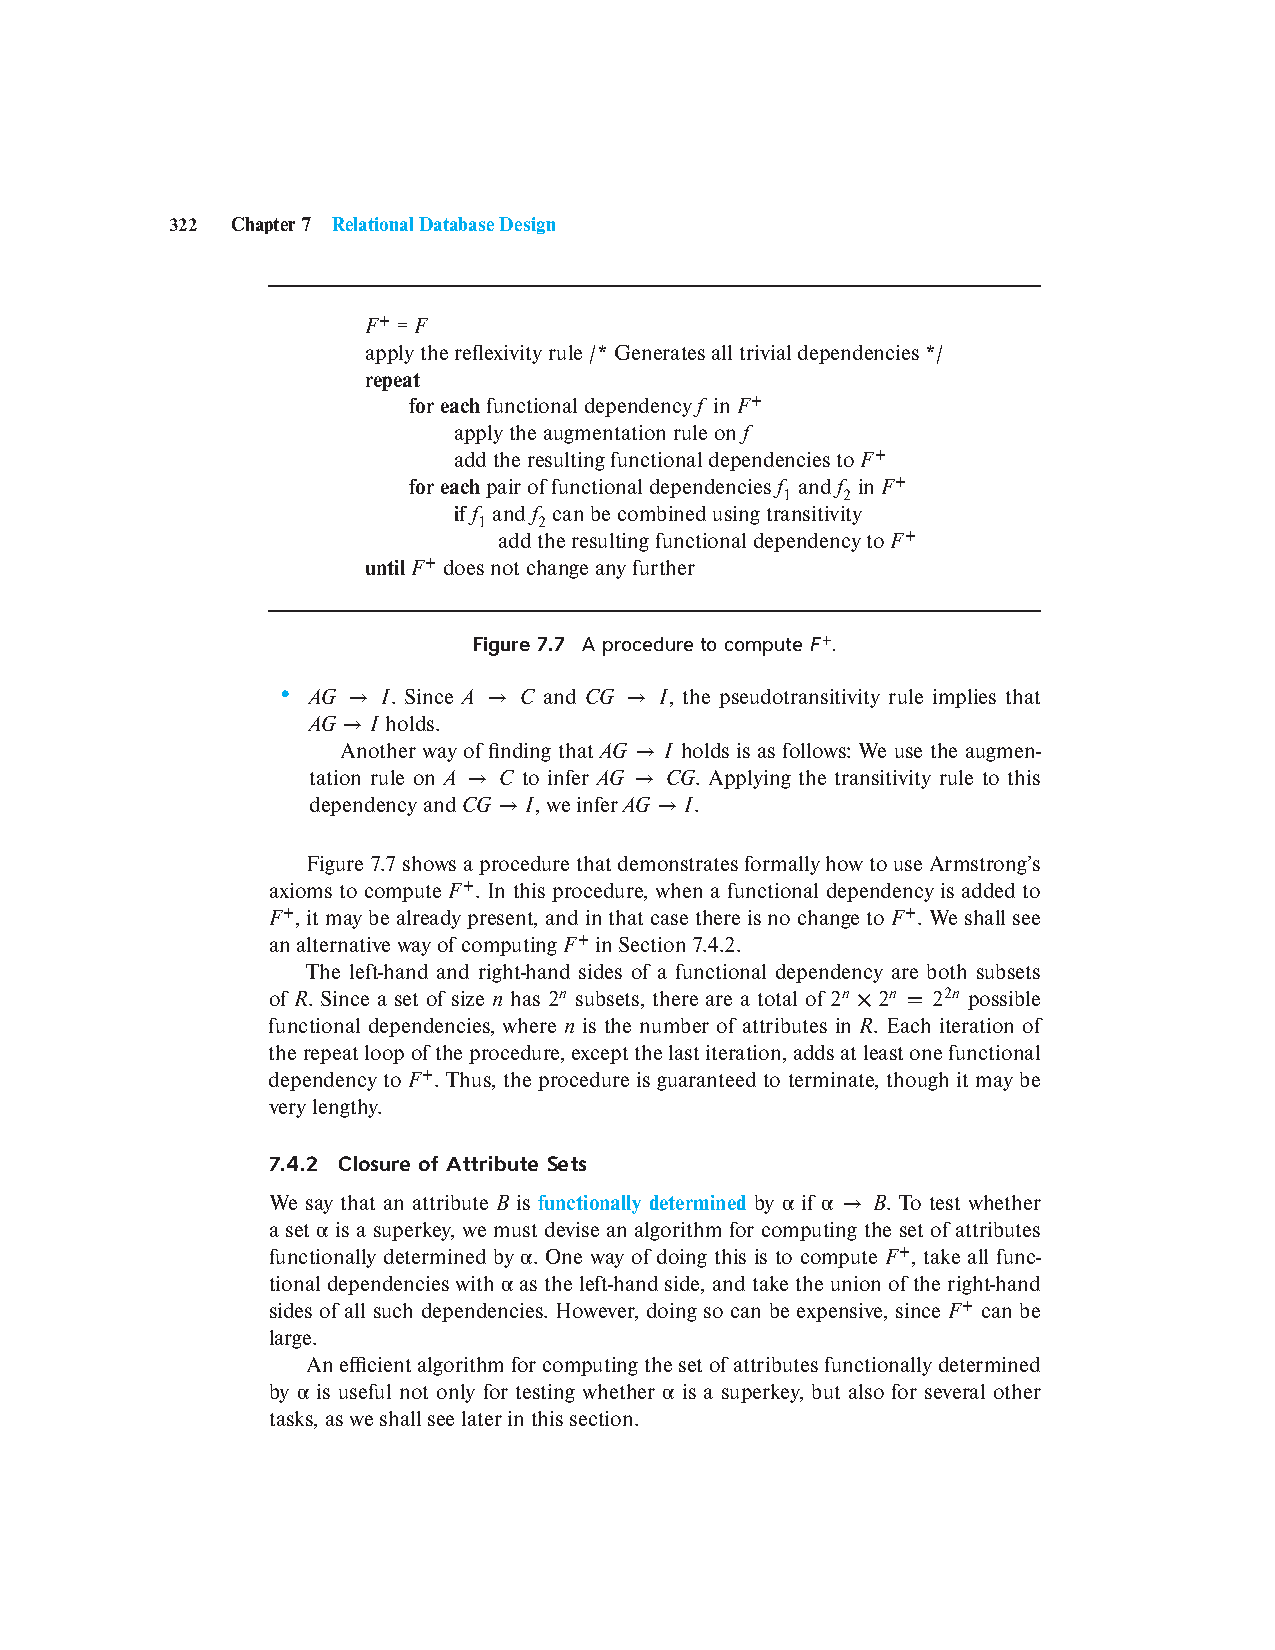
\includegraphics[width=\textwidth, trim={4cm 16.5cm 4cm 4.5cm}, clip]{figures/p322_Fplus_procedure}
\end{frame}

\begin{frame}{Closure of Attribute Sets}
    \begin{itemize}
        \item Given a set of attributes $\alpha$, define the closure of $\alpha$ under $F$ (denoted by $\alpha^+$) as the set of attributes that are functionally determined by $\alpha$ under $F$.
        \item Algorithm to compute $\alpha^+$, the closure of $\alpha$ under $F$:
    \end{itemize}
    \centering
    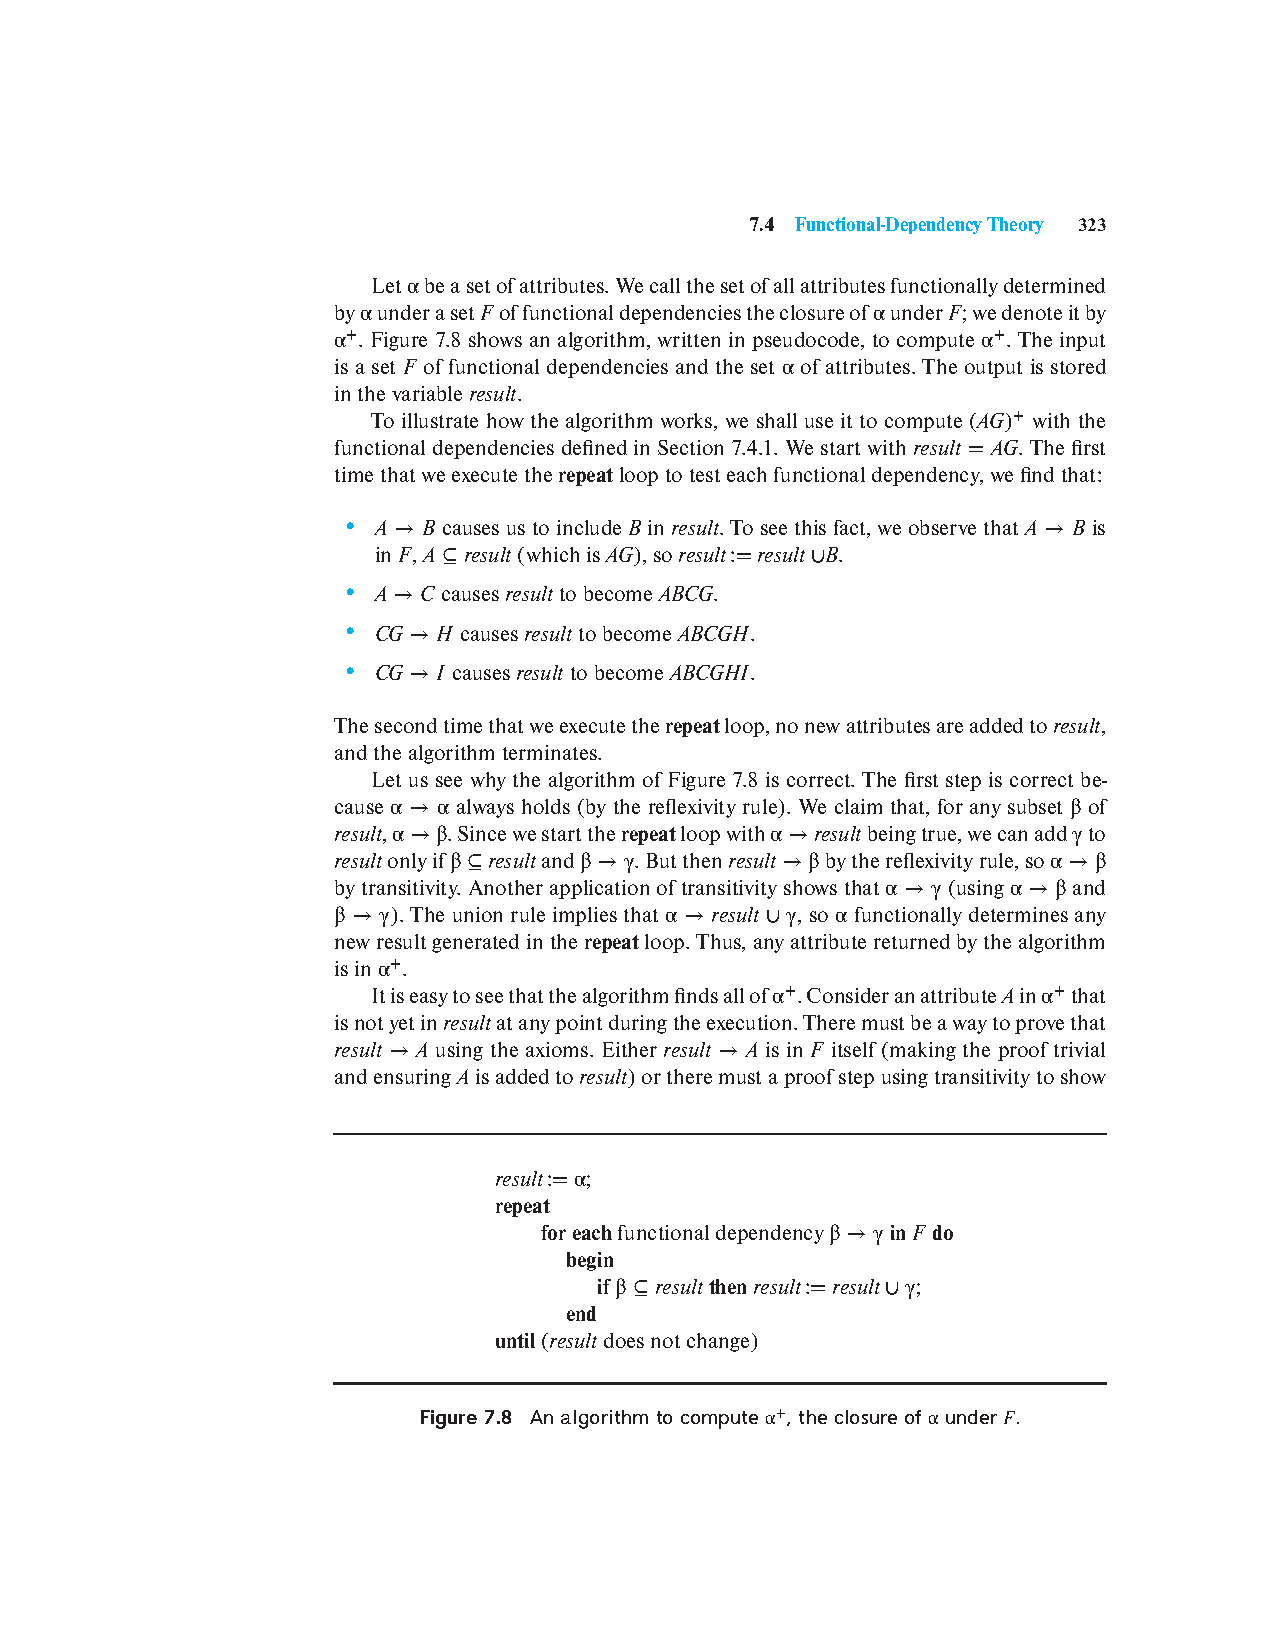
\includegraphics[width=0.9\textwidth, trim={6.5cm .75cm 3.5cm 19cm}, clip]{figures/p323_Aplus_procedure}
\end{frame}

\begin{frame}{Example of Attribute Set Closure}
    \footnotesize
    \begin{itemize}
        \item $R = (A, B, C, G, H, I)$
            \begin{equation*}
                \begin{align*}
                    F = \{  A   \rightarrow& B \\
                            A   \rightarrow& C \\
                            CG  \rightarrow& H \\
                            CG  \rightarrow& I \\
                            B   \rightarrow& H\} \\
                \end{align*}
            \end{equation*}
        \item $(AG)^+$
            \begin{enumerate}
                \item result = $AG$.
                \item result = $ABCG(A \rightarrow C$ and $A \rightarrow B)$.
                \item result = $ABCGH(CG \rightarrow H$ and $CG \subseteq AGBC)$.
                \item result = $ABCGHI(CG \rightarrow I$ and $CG \subseteq AGBCH)$.
            \end{enumerate}
        \item Is $AG$ a candidate key?
            \begin{enumerate}
                \item Is $AG$ a super key?
                    \begin{enumerate}
                        \item Does $AG \rightarrow R$? $==$ Is $R \supseteq (AG)^+$.
                    \end{enumerate}
                \item Is any subset of $AG$ a superkey?
                    \begin{enumerate}
                        \item Does $A \rightarrow R$? $==$ Is $R \supseteq (A)^+$.
                        \item Does $G \rightarrow R$? $==$ Is $R \supseteq (G)^+$.
                        \item In general: check for each subset of size $n-1$.
                    \end{enumerate}
            \end{enumerate}
    \end{itemize}
\end{frame}

\begin{frame}{Uses of Attribute Closure}
    There are several uses of the attribute closure algorithm:
    \begin{itemize}
        \item Testing for superkey
            \begin{itemize}
                \item To test if $\alpha$ is a superkey, we compute $\alpha^+$, and check if it contains all attributes of $R$.
            \end{itemize}
        \item Testing functional dependencies
            \begin{itemize}
                \item To check if a functional dependency $\alpha \rightarrow \beta$ holds (or, in other words, is in $F^+$), just check if $\beta \subseteq \alpha^+$.
                \item That is, we compute $\alpha^+$ by using attribute closure, and then check if it contains $\beta$.
            \end{itemize}
        \item Computing closure of F
            \begin{itemize}
                \item For each $\gamma \subseteq R$, we find the closure $\gamma+$, and for each $S \subseteq \gamma+$, we output a functional dependency $\gamma \rightarrow S$.
            \end{itemize}
    \end{itemize}
\end{frame}

\begin{frame}{Canonical Cover}
    \begin{itemize}
        \item When a user updates a relation, the database system must ensure that all functional dependencies in the set $F$ are still satisfied.
        \item If any FD is violated, the update is rolled back.
        \item To minimize the effort of checking for violations, the system can test a simplified set of $F$ with the same closure as the given set.
        \item This simplified set is termed the \textbf{canonical cover}.
        \item To define canonical cover we must first define \textbf{extraneous attributes}:
            \begin{itemize}
                \item An attribute of a functional dependency in $F$ is extraneous if we can remove it without changing $F^+$.
            \end{itemize}
    \end{itemize}
\end{frame}

\begin{frame}{Extraneous Attributes}
    \begin{itemize}
        \item Removing an attribute from the left side of a functional dependency could make it a stronger constraint.
            \begin{itemize}
                \item For example, if we have $AB \rightarrow C$ and remove $B$, we get the possibly stronger result $A \rightarrow C$. It may be stronger because $A \rightarrow C$ logically implies $AB \rightarrow C$, but $AB \rightarrow C$ does not, on its own, logically imply $A \rightarrow C$.
            \end{itemize}
        \item But, depending on what our set $F$ of functional dependencies happens to be, we may be able to remove $B$ from $AB \rightarrow C$ safely.
            \begin{itemize}
                \item For example, suppose that: $F = \{ AB \rightarrow C, A \rightarrow D, D \rightarrow C \}$
                \item Then we can show that $F$ logically implies $A \rightarrow C$, making extraneous in $AB \rightarrow C$.
            \end{itemize}
    \end{itemize}
\end{frame}

\begin{frame}{Extraneous Attributes (Cont.)}
    \begin{itemize}
        \item Removing an attribute from the right side of a functional dependency could make it a weaker constraint.
            \begin{itemize}
                \item For example, if we have $AB \rightarrow CD$ and remove $C$, we get the possibly weaker result $AB \rightarrow D$. It may be weaker because using just $AB \rightarrow D$, we can no longer infer $AB \rightarrow C$.
            \end{itemize}
        \item But, depending on what our set $F$ of functional dependencies happens to be, we may be able to remove $C$ from $AB \rightarrow CD$ safely.
            \begin{itemize}
                \item For example, suppose that: $F = \{ AB \rightarrow CD, A \rightarrow C \}$.
                \item Then we can show that even after replacing $AB \rightarrow CD$ by $AB \rightarrow D$, we can still infer $AB \rightarrow C$ and thus $AB \rightarrow CD$.
            \end{itemize}
    \end{itemize}
\end{frame}

\begin{frame}{Extraneous Attributes}
    \begin{itemize}
        \item An attribute of a functional dependency in $F$ is extraneous if we can remove it without changing $F^+$.
        \item Consider a set $F$ of functional dependencies and the functional dependency $\alpha \rightarrow \beta$ in $F$.
            \begin{itemize}
                \item \textbf{Remove from the left side}: Attribute $A$ is extraneous in $\alpha$ if:
                    \begin{itemize}
                        \item $A \in \alpha$ and
                        \item $F$ logically implies $(F - \{ \alpha \rightarrow \beta \}) \bigcup \{(\alpha - A) \rightarrow \beta \}$.
                    \end{itemize}
                \item \textbf{Remove from the right side}: Attribute $A$ is extraneous in $\beta$ if:
                    \begin{itemize}
                        \item $A \in \beta$ and
                        \item The set of functional dependencies $(F - \{ \alpha \rightarrow \beta \}) \bigcup \{ \alpha \rightarrow (\beta - A) \}$ logically implies $F$.
                    \end{itemize}
            \end{itemize}
    \end{itemize}
    \textbf{Note}: implication in the opposite direction is trivial in each of the cases above, since a ``stronger'' functional dependency always implies a weaker one
\end{frame}

\begin{frame}{Examples of Extraneous Attributes}
    \begin{itemize}
        \item Let
            $$
                F = \{ AB \rightarrow CD, A \rightarrow E, E \rightarrow C \}
            $$
        \item To check if $C$ is extraneous in $AB \rightarrow CD$, we:
            \begin{itemize}
                \item Compute the attribute closure of $AB$ under $F^\prime = \{ AB \rightarrow D, A \rightarrow E, E \rightarrow C \}$,
                    \begin{itemize}
                        \item Start with the initial set: $AB^+ = \{ A, B \}$
                        \item Apply the functional dependencies: \\
                            \( AB \rightarrow D \): Since \( A, B \in AB^+ \), add \( D \): $AB^+ = \{ A, B, D \}$ \\
                            \( A \rightarrow E \): Since \( A \in AB^+ \), add \( E \): $AB^+ = \{ A, B, D, E \}$ \\
                            \( E \rightarrow C \): Since \( E \in AB^+ \), add \( C \): $AB^+ = \{ A, B, D, E, C \}$
                    \end{itemize}
            \end{itemize}
    \end{itemize}
\end{frame}

\begin{frame}{Examples of Extraneous Attributes}
    \begin{itemize}
        \item Let
            $$
                F = \{ AB \rightarrow CD, A \rightarrow E, E \rightarrow C \}
            $$
        \item To check if $C$ is extraneous in $AB \rightarrow CD$, we:
            \begin{itemize}
                \item Compute the attribute closure of $AB$ under $F^\prime = \{ AB \rightarrow D, A \rightarrow E, E \rightarrow C \}$,
                \item The closure is $ABCDE$, which includes $CD$,
                \item This implies that $C$ is extraneous.
            \end{itemize}
    \end{itemize}
\end{frame}

\begin{frame}{Canonical Cover}
    \begin{itemize}
        \item A canonical cover for $F$ is a set of dependencies $F_c$ such that:
            \begin{itemize}
                \item $F$ logically implies all dependencies in $F_c$, and
                \item $F_c$ logically implies all dependencies in $F$, and
                \item No functional dependency in $F_c$ contains an extraneous attribute, and
                \item Each left side of functional dependency in $F_c$ is unique.  That is, there are no two dependencies in $F_c$
                    \begin{itemize}
                        \item $\alpha_1 \rightarrow \beta_1$ and $\alpha_2 \rightarrow \beta_2$ such that
                        \item $\alpha_1 = \alpha_2$
                    \end{itemize}
            \end{itemize}
    \end{itemize}
\end{frame}

\begin{frame}{Canonical Cover}
    To compute a canonical cover for F:
    \begin{center}
        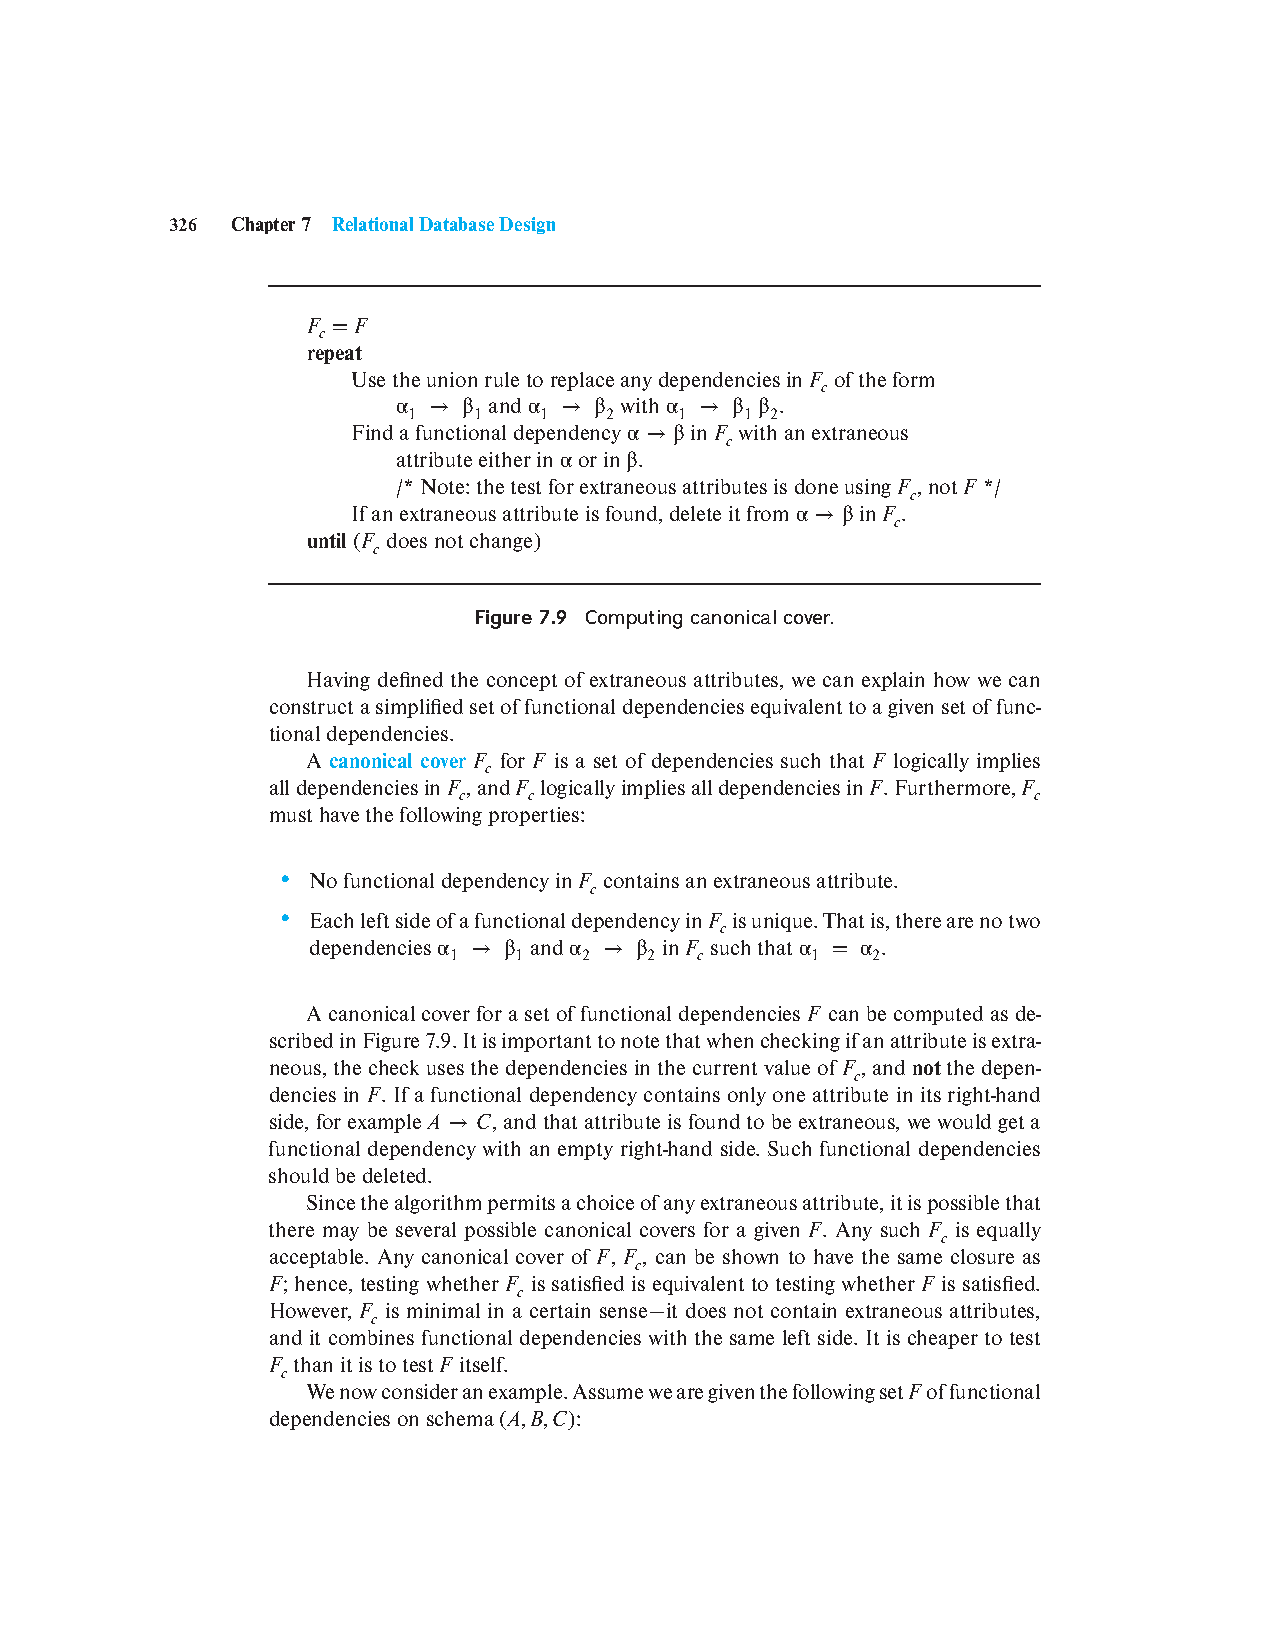
\includegraphics[width=\textwidth, trim={3.5cm 17cm 3.5cm 4.5cm}, clip]{figures/p326_Canonical}
    \end{center}
    \textbf{Note}: Union rule may become applicable after some extraneous attributes have been deleted, so it has to be re-applied.
\end{frame}

\begin{frame}{Example: Computing a Canonical Cover}
    \footnotesize
    \begin{itemize}
        \item $R = (A, B, C)$
            \begin{equation*}
                \begin{align*}
                    F = \{ A &\rightarrow BC \\
                            B &\rightarrow C \\
                            A &\rightarrow B \\
                            AB &\rightarrow C \}
                \end{align*}
            \end{equation*}
        \item Combine $A \rightarrow BC$ and $A \rightarrow B$ into $A \rightarrow BC$
            \begin{itemize}
                \item Set is now $\{ A \rightarrow BC, B \rightarrow C, AB \rightarrow C \}$
            \end{itemize}
        \item $A$ is extraneous in $AB \rightarrow C$
            \begin{itemize}
                \item Check if the result of deleting $A$ from $AB \rightarrow C$ is implied by the other dependencies ($B \rightarrow C$ is already present!).
                \item Set is now $\{ A \rightarrow BC, B \rightarrow C \}$
            \end{itemize}
        \item $C$ is extraneous in $A \rightarrow BC$
            \begin{itemize}
                \item Check if $A \rightarrow C$ is logically implied by $A \rightarrow B$ and the other dependencies (using transitivity on $A \rightarrow B$ and $B \rightarrow C$).
            \end{itemize}
        \item The canonical cover is:
            \begin{equation*}
                \begin{align*}
                    A &\rightarrow B \\
                    B &\rightarrow C
                \end{align*}
            \end{equation*}
    \end{itemize}
\end{frame}

\begin{frame}{Dependency Preservation}
    \begin{itemize}
        \item Let $F_i$ be the set of dependencies $F^+$ that include only attributes in $R_i$.
            \begin{itemize}
                \item A decomposition is dependency preserving, if
                    $$
                        (F_1 \bigcup F_2 \bigcup \cdots \bigcup F_n )^+ = F^+
                    $$
            \end{itemize}

        \item Using the above definition, testing for \textbf{dependency preservation} take exponential time.
        \item Not that if a decomposition is NOT dependency preserving then checking updates for violation of functional dependencies may require computing joins, which is expensive.
    \end{itemize}
\end{frame}

\begin{frame}{Dependency Preservation (Cont.)}
    \begin{itemize}
        \item Let $F$ be the set of dependencies on schema $R$ and let $R_1, R_2, \ldots, R_n$ be a decomposition of $R$.
        \item The restriction of $F$ to $R_i$ is the set $F_i$ of all functional dependencies in $F^+$ that include only attributes of $R_i$.
        \item Since all functional dependencies in a restriction involve attributes of only one relation schema, it is possible to test such a dependency for satisfaction by checking only one relation.
        \item Note that the definition of restriction uses all dependencies in $F^+$, not just those in $F$.
        \item The set of restrictions $F_1, F_2 , \ldots, F_n$ is the set of functional dependencies that can be checked efficiently.
    \end{itemize}
\end{frame}

\begin{frame}{Testing for Dependency Preservation}
    \begin{itemize}
        \item To check if a dependency $\alpha \rightarrow \beta$ is preserved in a decomposition of $R$ into $R_1, R_2, \ldots, R_n$, we apply the following test (with attribute closure done with respect to $F$):
            \begin{center}
                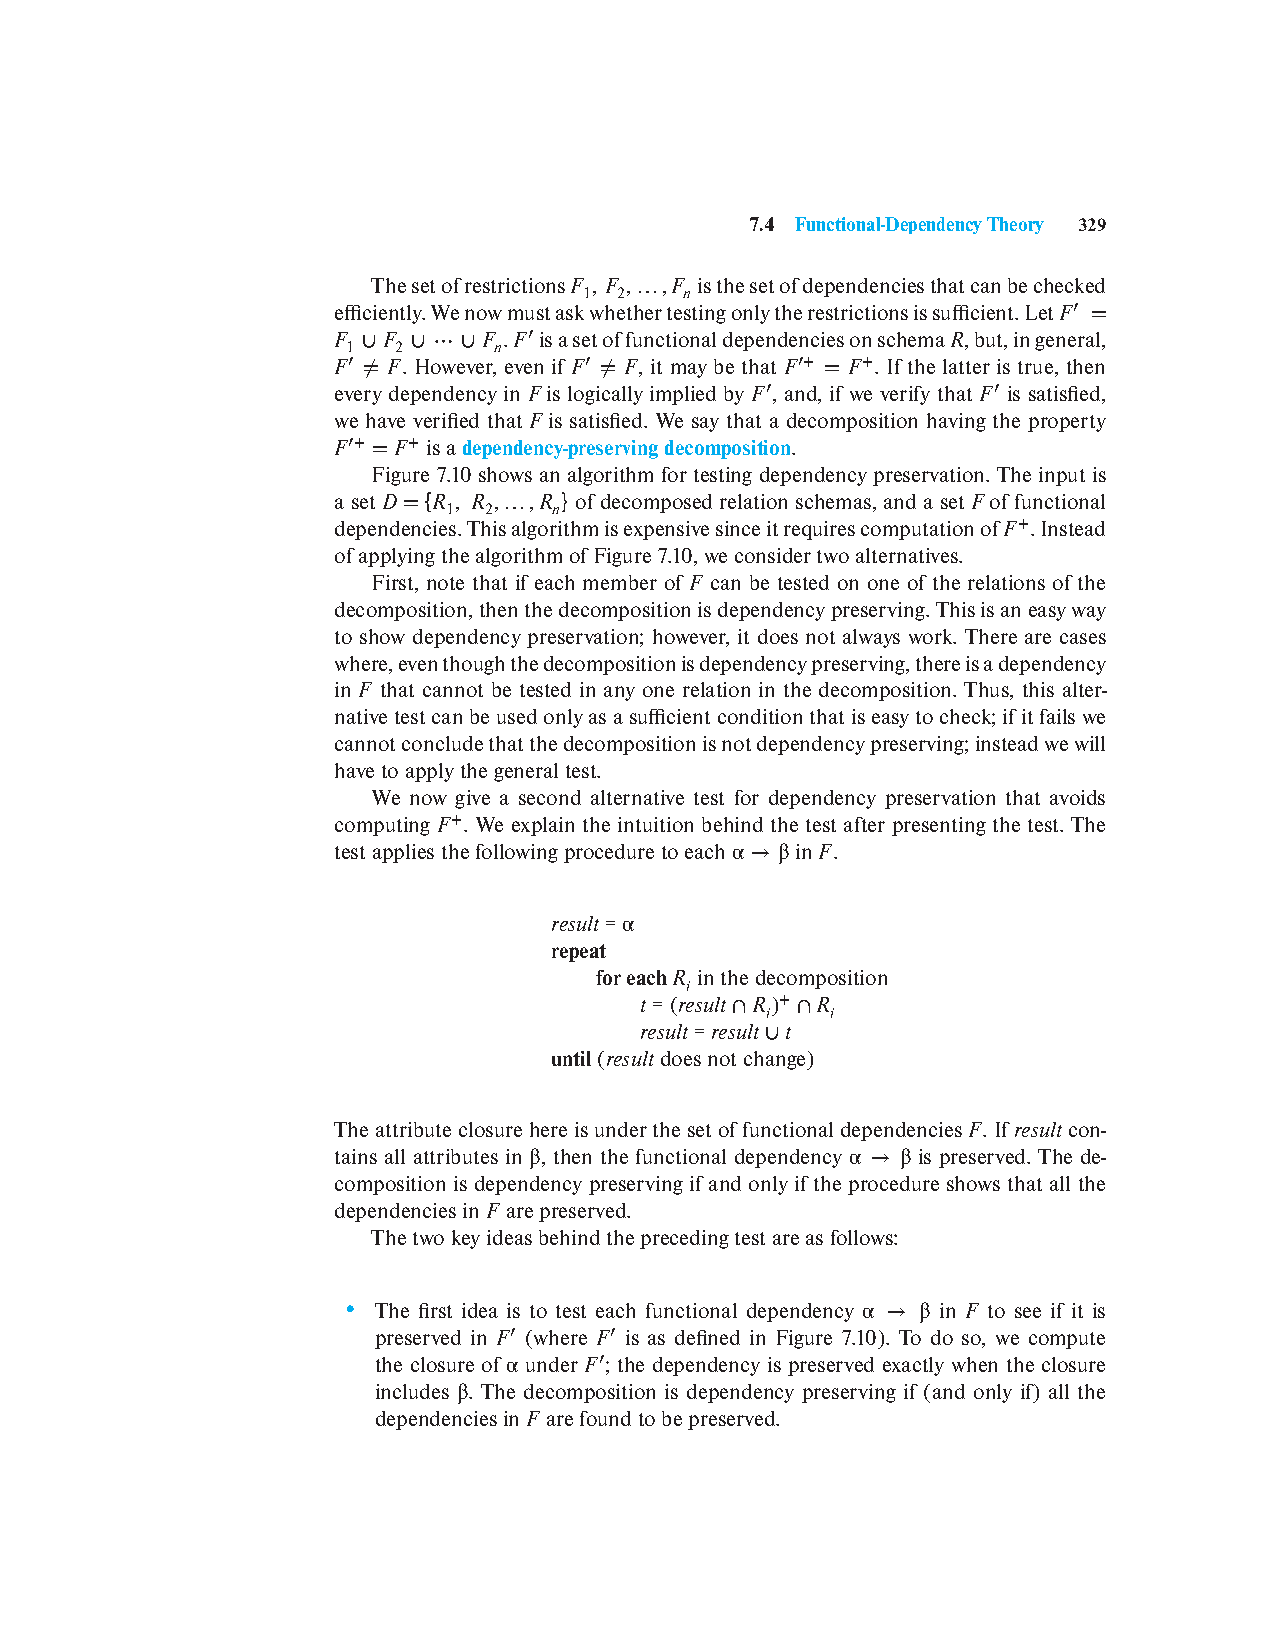
\includegraphics[width=\textwidth, trim={5cm 9.5cm 2.5cm 15.5cm}, clip]{figures/p329_Preserving}
            \end{center}
        \item We apply the test on all dependencies in $F$ to check if a decomposition is dependency preserving.
        \item This procedure takes polynomial time, instead of the exponential time required to compute $F^+$ and $(F_1 \bigcup F_2 \bigcup \ldots  F_n)+$.
    \end{itemize}
\end{frame}

\begin{frame}{Example}
    \begin{itemize}
        \item $R = (A, B, C)$
            \begin{equation*}
                \begin{align*}
                    F = \{ A &\rightarrow B \\
                            B &\rightarrow C \} \\
                    Key = \{ A \}
                \end{align*}
            \end{equation*}
        \item $R$ is not in BCNF.
        \item Decomposition $R_1 = (A, B)$, $R_2 = (B, C)$:
            \begin{itemize}
                \item $R_1$ and $R_2$ in BCNF.
                \item Lossless-join decomposition.
                \item Dependency preserving.
            \end{itemize}
    \end{itemize}
\end{frame}

\section{Algorithms for Decomposition using Functional Dependencies}

\begin{frame}{Testing for BCNF}
    \footnotesize
    \begin{itemize}
        \item To check if a non-trivial dependency $\alpha \rightarrow \beta$ causes a violation of BCNF:
            \begin{enumerate}
                \item compute $\alpha^+$ (the attribute closure of $\alpha$), and
                \item verify that it includes all attributes of $R$, that is, it is a superkey of $R$.
            \end{enumerate}
        \item \textbf{Simplified test}: To check if a relation schema $R$ is in BCNF, it suffices to check only the dependencies in the given set $F$ for violation of BCNF, rather than checking all dependencies in $F^+$.
            \begin{itemize}
                \item If none of the dependencies in $F$ causes a violation of BCNF, then none of the dependencies in $F^+$ will cause a violation of BCNF either ...
            \end{itemize}
    \end{itemize}
\end{frame}

\begin{frame}{Testing for BCNF (Cont.)}
    \footnotesize
    \begin{itemize}
        \item However, \textbf{simplified test} using only $F$ is incorrect when testing a relation in a decomposition of $R$:\\
            Consider $R = (A, B, C, D, E)$, with $F = \{ A \rightarrow B, BC \rightarrow D \}$
            \begin{itemize}
                \item Decompose $R$ into $R_1 = (A,B)$ and $R_2 = (A,C,D,E)$,
                \item Neither of the dependencies in $F$ contain only attributes from $(A,C,D,E)$ so we might be mislead into thinking $R_2$ satisfies BCNF.
                \item In fact, dependency $AC \rightarrow D$ in $F^+$ shows $R_2$ is not in BCNF.
            \end{itemize}
    \end{itemize}
\end{frame}

\begin{frame}{Testing Decomposition for BCNF}
    \begin{itemize}
        \item To check if a relation Ri in a decomposition of R is in BCNF,
            \begin{itemize}
                \item Either test $R_i$ for BCNF with respect to the restriction of $F^+$ to $R_i$ (that is, all FDs in $F^+$ that contain only attributes from $R_i$)
                \item or use the original set of dependencies $F$ that hold on $R$, but with the following test:
                    \begin{itemize}
                        \item for every set of attributes $\alpha \subseteq R_i$, check that $\alpha^+$ (the attribute closure of $\alpha$) either includes no attribute of $R_i - \alpha$, or includes all attributes of $R_i$.
                    \end{itemize}
                \item If the condition is violated by some $\alpha \rightarrow \beta$ in $F^+$, the dependency:
                    $$
                        \alpha \rightarrow (\alpha^+ - \alpha) \bigcap R_i
                    $$
                    can be shown to hold on $R_i$, and $R_i$ violates BCNF.
                \item We use above dependency to decompose $R_i$.
            \end{itemize}
    \end{itemize}
\end{frame}

\begin{frame}{BCNF Decomposition Algorithm}
    \begin{center}
        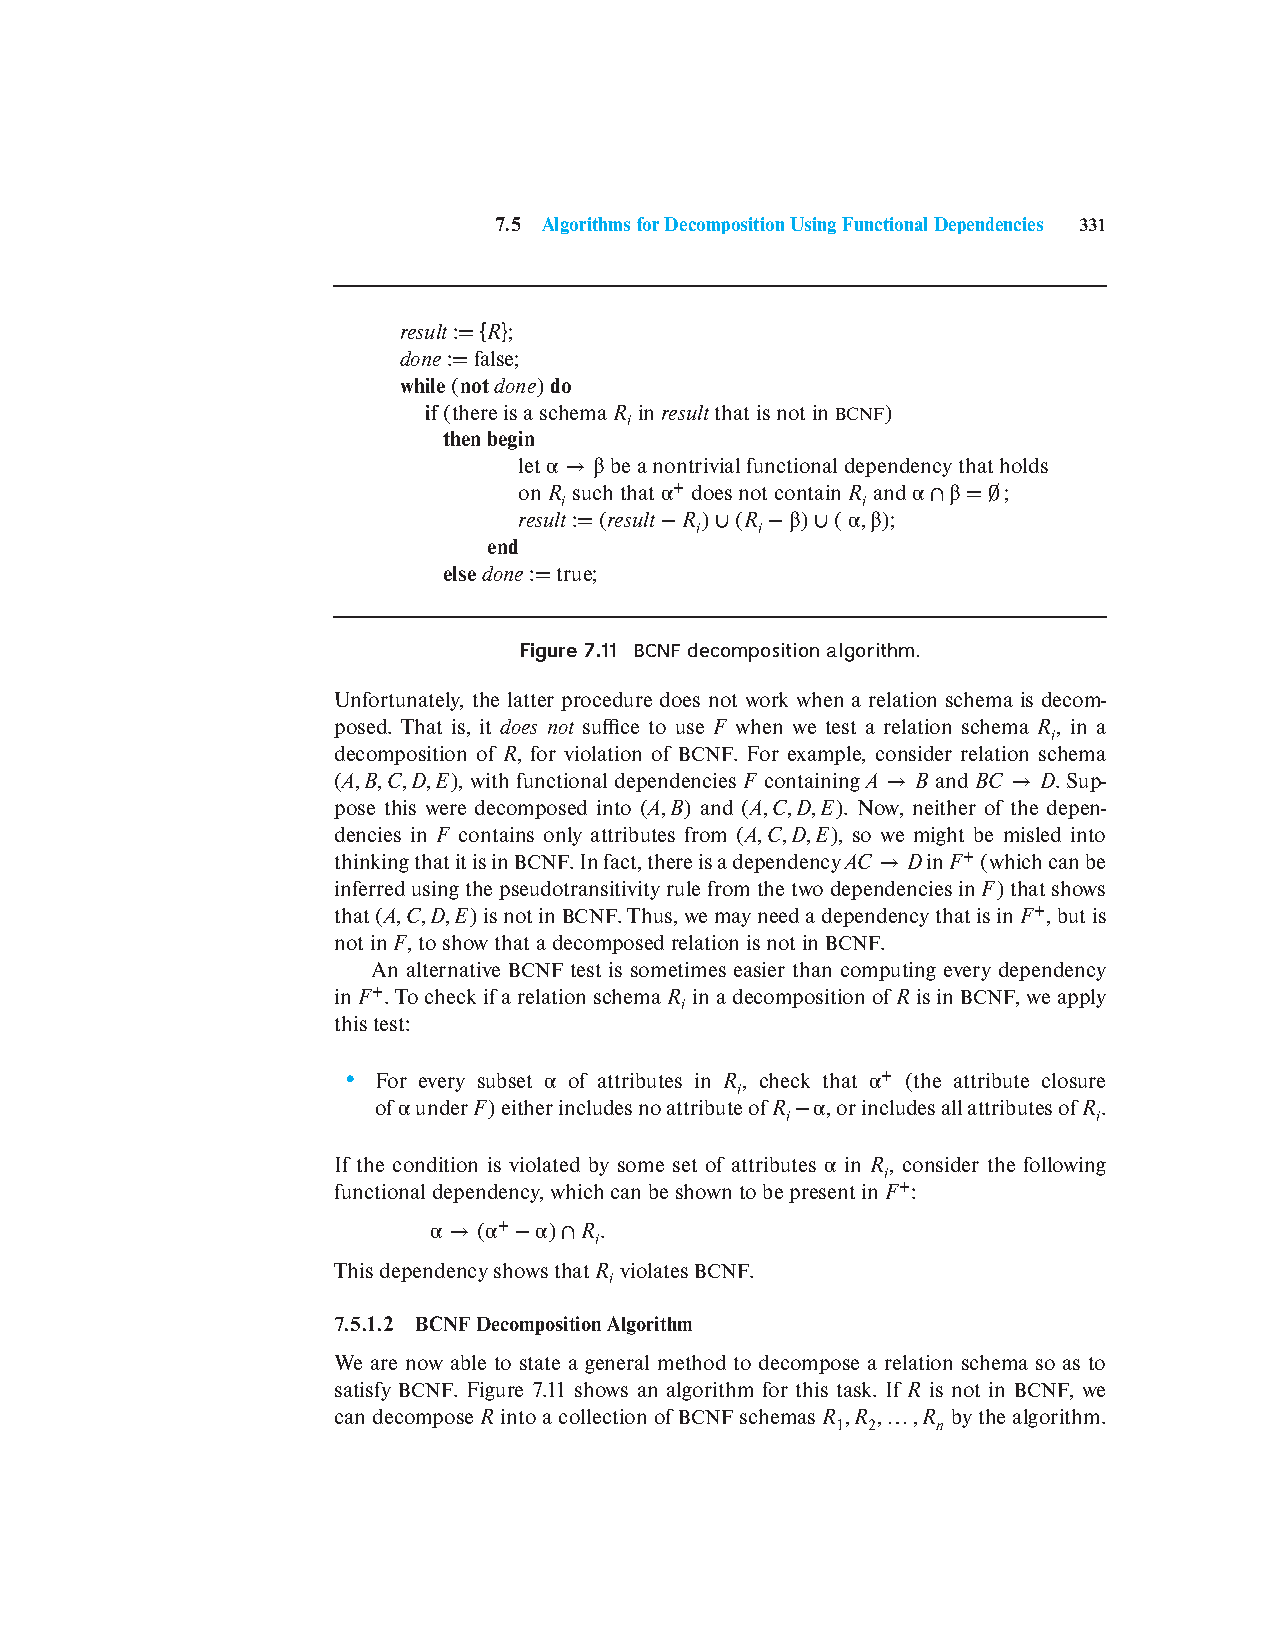
\includegraphics[width=\textwidth, trim={5.5cm 16.5cm 3cm 4.5cm}, clip]{figures/p331_Decomposition_BCNF}
    \end{center}
    \textbf{Note}: each $R_i$ is in BCNF, and decomposition is lossless-join.
\end{frame}

\begin{frame}[fragile]{Example of BCNF Decomposition}
    \footnotesize
    \begin{itemize}
        \item
            \begin{verbatim}
class (course_id, title, dept_name, credits, sec_id,
    semester, year, building, room_number, capacity,
    time_slot_id)
            \end{verbatim}
            \vspace{-8mm}
            \begin{equation*}
                \begin{align*}
                    F = \{
                        course\_id &\rightarrow title, dept\_name, credits \\
                        building, room\_number &\rightarrow capacity \\
                        course\_id, sec\_id, semester, year &\rightarrow building, room\_number, time\_slot\_id \}
                \end{align*}
            \end{equation*}
        \item A candidate key \verb|{course_id, sec_id, semester, year}|.
        \item BCNF Decomposition:
            \begin{itemize}
                \item $course\_id \rightarrow title, dept\_name, credits$ holds but $course\_id$ is not a superkey.
                \item We replace \texttt{class} by:
                    \begin{itemize}
                        \item \verb|course(course_id, title, dept_name, credits)|
                        \item \begin{verbatim}
class-1 (course_id, sec_id, semester, year, building,
    room_number, capacity, time_slot_id)
                            \end{verbatim}
                    \end{itemize}
            \end{itemize}
    \end{itemize}
\end{frame}

\begin{frame}[fragile]{Example of BCNF Decomposition (Cont.)}
    \footnotesize
    \begin{itemize}
        \item course is in BCNF.
            \begin{itemize}
                \item How do we know this?
            \end{itemize}
        \item $building, room\_number \rightarrow capacity$ holds on \texttt{class-1}
            \begin{itemize}
                \item but $\{ building, room\_number \}$ is not a superkey for \texttt{class-1}.
                \item We replace \texttt{class-1} by:
                    \begin{itemize}
                        \item \verb|classroom(building, room_number, capacity)|
                        \item \begin{verbatim}
section (course_id, sec_id, semester, year, building,
    room_number, time_slot_id)
                              \end{verbatim}
                    \end{itemize}
            \end{itemize}
    \end{itemize}
\end{frame}

\begin{frame}{Third Normal Form}
    \begin{itemize}
        \item There are some situations where:
            \begin{itemize}
                \item BCNF is not dependency preserving, and
                \item efficient checking for FD violation on updates is important.
            \end{itemize}
        \item Solution: define a weaker normal form, called Third Normal Form (3NF)
            \begin{itemize}
                \item Allows some redundancy (with resultant problems; we will see examples later)
                \item But functional dependencies can be checked on individual relations without computing a join.
                \item There is always a lossless-join, dependency- preserving decomposition into 3NF.
            \end{itemize}
    \end{itemize}
\end{frame}

% \begin{frame}[fragile]{3NF Example}
%     \begin{itemize}
%         \item Relation \texttt{dept\_advisor}:
%             \begin{itemize}
%                 \item \verb|dept_advisor (s_ID, i_ID, dept_name)| \\
%                     $F = \{ s\_ID, dept\_name \rightarrow i\_ID, i\_ID \rightarrow dept\_name \}$
%                 \item Two candidate keys: $\{ s\_ID, dept\_name \}$, and $\{ i\_ID, s\_ID \}$
%                 \item $R$ is in 3NF.
%                     \begin{itemize}
%                         \item $s\_ID, dept\_name \rightarrow i\_ID, s\_ID$ \\
%                             • $dept\_name$ is a superkey
%                         \item $i\_ID \rightarrow dept\_name$ \\
%                             • $dept\_name$ is contained in a candidate key
%                     \end{itemize}
%             \end{itemize}
%     \end{itemize}
% \end{frame}

\begin{frame}{Testing for 3NF}
    \begin{itemize}
        \item Need to check only FDs in $F$, need not check all FDs in $F^+$.
        \item Use attribute closure to check for each dependency $\alpha \rightarrow \beta$, if $\alpha$ is a superkey.
        \item If $\alpha$ is not a superkey, we have to verify if each attribute in $\beta$ is contained in a candidate key of $R$:
            \begin{itemize}
                \item This test is rather more expensive, since it involve finding candidate keys.
                \item Testing for 3NF has been shown to be NP-hard.
                \item Interestingly, decomposition into third normal form (described shortly) can be done in polynomial time.
            \end{itemize}
    \end{itemize}
\end{frame}

\begin{frame}{3NF Decomposition Algorithm}
    \begin{center}
        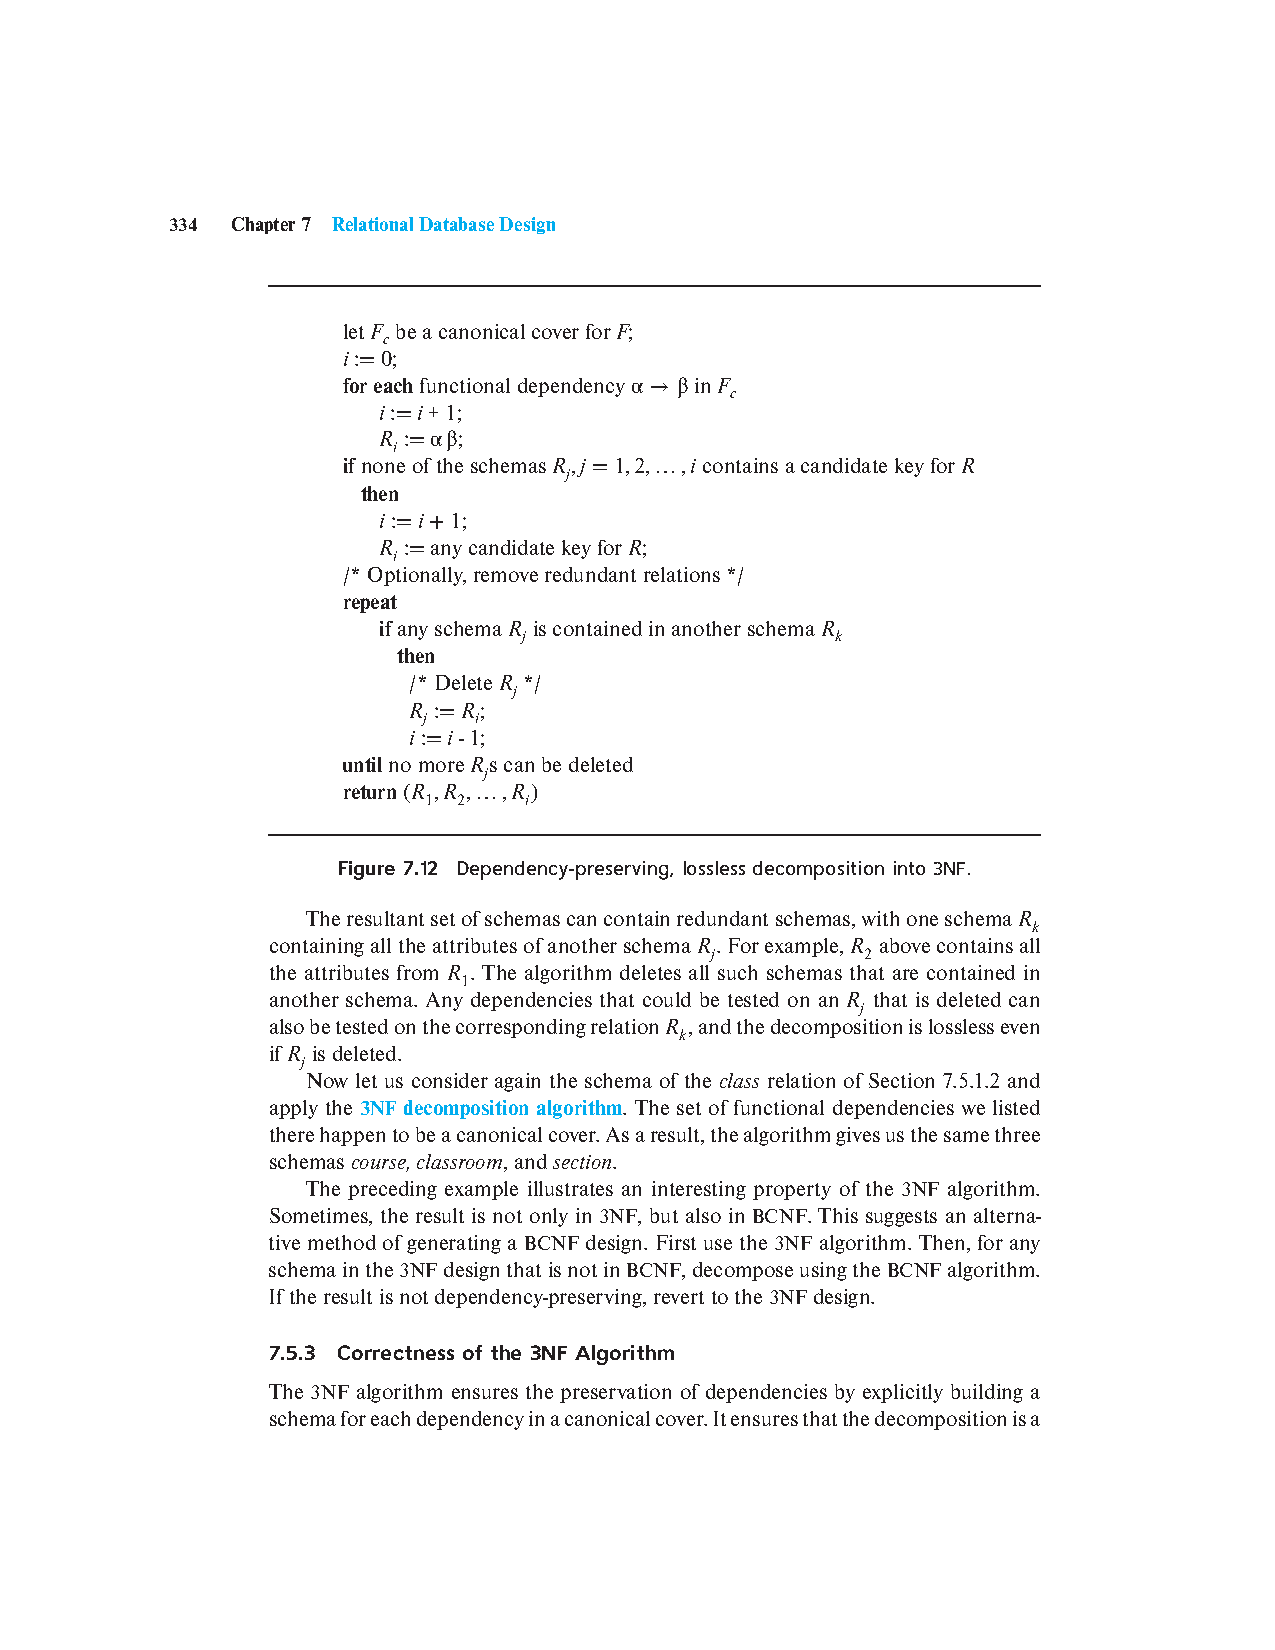
\includegraphics[width=0.9\textwidth, trim={5.5cm 12.75cm 3cm 4.5cm}, clip]{figures/p334_Decomposition_3NF}
    \end{center}
\end{frame}

\begin{frame}{3NF Decomposition Algorithm (Cont.)}
    \begin{itemize}
        \item Above algorithm ensures:
        \begin{itemize}
            \item each relation schema $R_i$ is in 3NF
            \item decomposition is dependency preserving and lossless-join
            \item Proof of correctness is in the Book.
        \end{itemize}
    \end{itemize}
\end{frame}

\begin{frame}[fragile]{3NF Decomposition: An Example}
    \footnotesize
    \begin{itemize}
        \item Relation schema:
            \begin{verbatim}
cust_banker_branch = (customer_id, employee_id, branch_name,
    type)
            \end{verbatim}
            \vspace{-5mm}
        \item The functional dependencies for this relation schema are:
            \begin{equation*}
                \begin{align*}
                    customer\_id, employee\_id &\rightarrow branch\_name, type \\
                    employee\_id &\rightarrow branch\_name \\
                    customer\_id, branch\_name &\rightarrow employee\_id \\
                \end{align*}
            \end{equation*}
        \item We first compute a canonical cover:
            \begin{itemize}
                \item $branch\_name$ is extraneous in the r.h.s. of the $1^{st}$ dependency.
                \item No other attribute is extraneous, so we get
                    \begin{equation*}
                        \begin{align*}
                            F_C = \{ customer\_id, employee\_id & \rightarrow type, \\
                                  employee\_id & \rightarrow branch\_name, \\
                                  customer\_id, branch\_name & \rightarrow employee\_id \}
                        \end{align*}
                    \end{equation*}
            \end{itemize}
    \end{itemize}
\end{frame}

\begin{frame}[fragile]{3NF Decomposition: An Example}
    \footnotesize
    \begin{itemize}
        \item The \textbf{for} loop generates following 3NF schema: \\
            \quad $(customer\_id, employee\_id, type)$ \\
            \quad $(employee\_id, branch\_name)$ \\
            \quad $(customer\_id, branch\_name, employee\_id)$
                \begin{itemize}
                    \item Observe that $(customer\_id, employee\_id, type)$ contains a candidate key of the original schema, so no further relation schema needs be added.
                \end{itemize}
        \item At end of for loop, detect and delete schemas, such as $(employee\_id, branch\_name)$, which are subsets of other schemas.
            \begin{itemize}
                \item result will not depend on the order in which FDs are considered.
            \end{itemize}
        \item The resultant simplified 3NF schema is: \\
            \quad (customer\_id, employee\_id, type) \\
            \quad (customer\_id, branch\_name, employee\_id)
    \end{itemize}
\end{frame}

\begin{frame}{Comparison of BCNF and 3NF}
    \begin{itemize}
        \item It is always possible to decompose a relation into a set of relations that are in 3NF such that:
            \begin{itemize}
                \item The decomposition is lossless.
                \item The dependencies are preserved.
            \end{itemize}
        \item It is always possible to decompose a relation into a set of relations that are in BCNF such that:
            \begin{itemize}
                \item The decomposition is lossless.
                \item It may not be possible to preserve dependencies.
            \end{itemize}
    \end{itemize}
\end{frame}


\begin{frame}{Design Goals}
    \begin{itemize}
        \item Goal for a relational database design is:
            \begin{itemize}
                \item BCNF.
                \item Lossless join.
                \item Dependency preservation.
            \end{itemize}
        \item If we cannot achieve this, we accept one of
            \begin{itemize}
                \item Lack of dependency preservation.
                \item Redundancy due to use of 3NF.
            \end{itemize}
        \item Interestingly, SQL does not provide a direct way of specifying functional dependencies other than superkeys. Can specify FDs using assertions, but they are expensive to test, (and currently not supported by any of the widely used databases!)
        \item Even if we had a dependency preserving decomposition, using SQL we would not be able to efficiently test a functional dependency whose left hand side is not a key.
    \end{itemize}
\end{frame}

\section{Decomposition Using Multivalued Dependencies}

\begin{frame}{Multivalued Dependencies (MVDs)}
    \begin{itemize}
        \item Suppose we record names of children, and phone numbers for instructors: \\
            \quad $inst\_child(ID, child\_name)$ \\
            \quad $inst\_phone(ID, phone\_number)$
        \item If we were to combine these schemas to get
            \begin{itemize}
                \item $inst\_info(ID, child\_name, phone\_number)$
                \item Example data:\\
                    \quad (99999, David, 512-555-1234) \\
                    \quad (99999, David, 512-555-4321) \\
                    \quad (99999, William, 512-555-1234) \\
                    \quad (99999, William, 512-555-4321)
            \end{itemize}
        \item This relation is in BCNF.  \textbf{Why?}
    \end{itemize}
\end{frame}

\begin{frame}{Multivalued Dependencies}
    Let R be a relation schema and let $\alpha \subseteq R$ and $\beta \subseteq R$. The multivalued dependency
        $$
            \alpha \twoheadrightarrow \beta
        $$
    holds on $R$ if in any legal relation $r(R)$, for all pairs for tuples $t_1$ and $t_2$ in $r$ such that $t_1[\alpha] = t_2[\alpha]$, there exist tuples $t_3$ and $t_4$ in $r$ such that:
        \begin{equation*}
            \begin{align*}
                t_1[\alpha] = t_2[\alpha] &= t_3[\alpha] = t_4[\alpha] \\
                t_3[\beta] &= t_1[\beta] \\
                t_3[R - \beta] &= t_2[R - \beta] \\
                t_4[\beta] &= t_2[\beta] \\
                t_4[R - \beta] &= t_1[R - \beta] \\
            \end{align*}
        \end{equation*}
\end{frame}

\begin{frame}{MVD -- Tabular representation}
    \begin{center}
        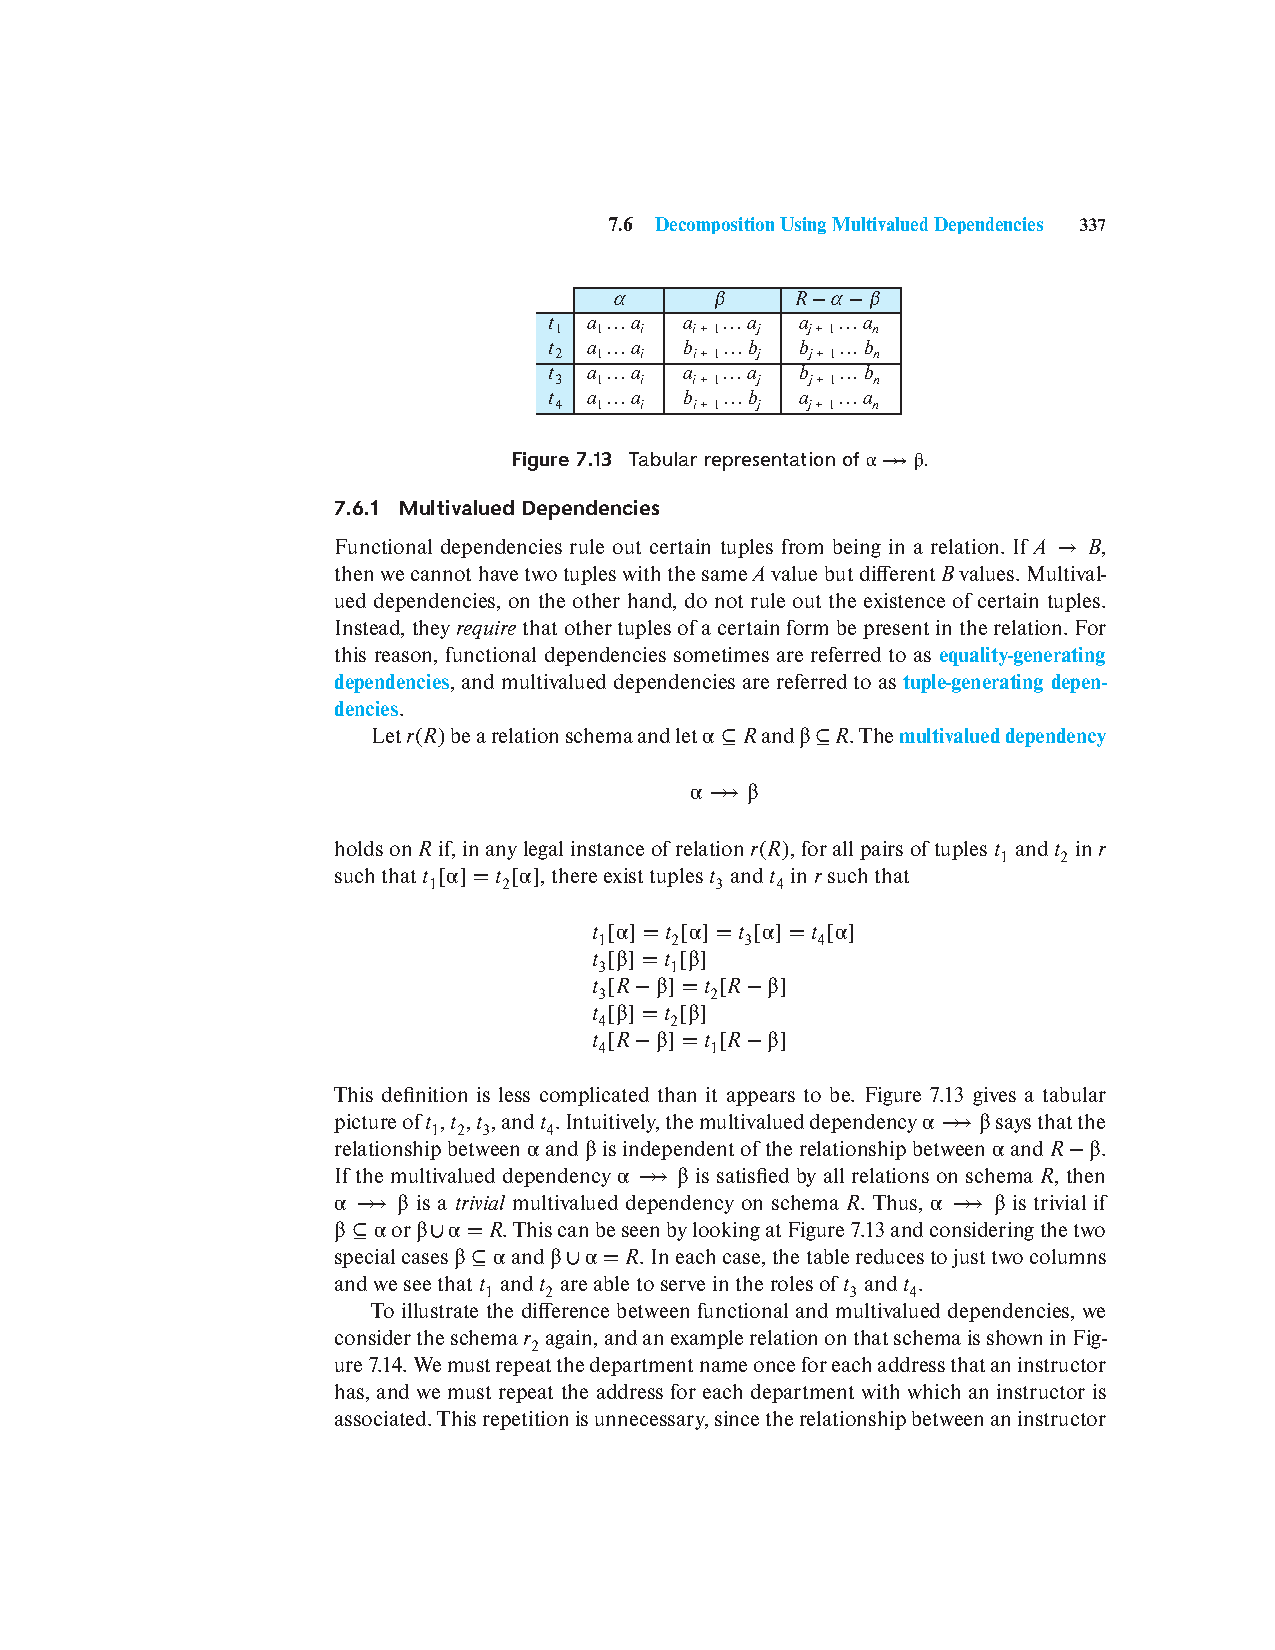
\includegraphics[width=\textwidth, trim={7.5cm 19.75cm 5cm 4.5cm}, clip]{figures/p337_tabular}
    \end{center}
\end{frame}

\begin{frame}{MVD (Cont.)}
    \begin{itemize}
        \item Let $R$ be a relation schema with a set of attributes that are partitioned into 3 nonempty subsets: $Y, Z, W$.
        \item We say that $Y \twoheadrightarrow Z$ ($Y$ multidetermines $Z$) if and only if for all possible relations $r(R)$:
            \begin{equation*}
                < y_1, z_1, w_1 > \in r \text{ and } < y_1, z_2, w_2 > \in r
            \end{equation*}
            then
            \begin{equation*}
                < y_1, z_1, w_2 > \in r \text{ and } < y_1, z_2, w_1 > \in r
            \end{equation*}
        \item Note that since the behavior of $Z$ and $W$ are identical it follows that
            \begin{equation*}
                Y \twoheadrightarrow Z \text{ if } Y \twoheadrightarrow W
            \end{equation*}
    \end{itemize}

\end{frame}

\begin{frame}{Example}
    \begin{itemize}
        \item In our example: \\
            \quad $ID \twoheadrightarrow child\_name$ \\
            \quad $ID \twoheadrightarrow phone\_number$ \\

        \item The above formal definition is supposed to formalize the notion that given a particular value of $Y(ID)$ it has associated with it a set of values of $Z(child\_name)$ and a set of values of $W(phone\_number)$, and these two sets are in some sense independent of each other.

        \item Note:
            \begin{itemize}
                \item If $Y \rightarrow Z$ then $Y \twoheadrightarrow Z$
                \item Indeed we have (in above notation) $Z_1 = Z_2$ \\
                    The claim follows.
            \end{itemize}
    \end{itemize}
\end{frame}

\begin{frame}{Use of Multivalued Dependencies}
    \begin{itemize}
        \item We use multivalued dependencies in two ways:
            \begin{enumerate}
                \item To test relations to \textbf{determine} whether they are legal under a given set of functional and multivalued dependencies.
                \item To specify \textbf{constraints} on the set of legal relations. We shall concern ourselves only with relations that satisfy a given set of functional and multivalued dependencies.
            \end{enumerate}

        \item If a relation $r$ fails to satisfy a given multivalued dependency, we can construct a relations $r^\prime$ that does satisfy the multivalued dependency by adding tuples to $r$.
    \end{itemize}
\end{frame}

\begin{frame}{Theory of MVDs}
    \begin{itemize}
        \item From the definition of multivalued dependency, we can derive the following rule:
            \begin{equation*}
                \text{ If } \alpha \rightarrow \beta \text{, then } \alpha \twoheadrightarrow \beta
            \end{equation*}
            That is, every functional dependency is also a multivalued dependency.

        \item The closure $D^+$ of $D$ is the set of all functional and multivalued dependencies logically implied by $D$.
            \begin{itemize}
                \item We can compute $D+$ from $D$, using the formal definitions of functional dependencies and multivalued dependencies.
                \item We can manage with such reasoning for very simple multivalued dependencies, which seem to be most common in practice
                \item For complex dependencies, it is better to reason about sets of dependencies using a system of inference rules (\href{https://db-book.com/online-chapters-dir/28.pdf}{Section 28.1.1}).
            \end{itemize}
    \end{itemize}
\end{frame}

\section{More Normal Form}

\begin{frame}{Fourth Normal Form}
    \begin{itemize}
        \item A relation schema $R$ is in \textbf{4NF} with respect to a set $D$ of functional and multivalued dependencies if for all multivalued dependencies in $D^+$ of the form $\alpha \twoheadrightarrow \beta$, where $\alpha \subseteq R$ and $\beta \subseteq R$, at least one of the following hold:
            \begin{itemize}
                \item $\alpha \twoheadrightarrow \beta$ is trivial (i.e., $\beta \subseteq \alpha$ or $\alpha \bigcup \beta = R$).
                \item $\alpha$ is a superkey for schema $R$.
            \end{itemize}
        \item If a relation is in 4NF it is in BCNF.
    \end{itemize}
\end{frame}

\begin{frame}{Restriction of Multivalued Dependencies}
    The restriction of $D$ to $R_i$ is the set $D_i$ consisting of:
        \begin{itemize}
            \item All functional dependencies in $D^+$ that include only attributes of $R_i$
            \item All multivalued dependencies of the form:
                $$
                    \alpha \twoheadrightarrow (\beta \bigcap R_i)
                $$
                where $\alpha \subseteq R_i$ and $\alpha \twoheadrightarrow \beta$ is in $D^+$.
        \end{itemize}
\end{frame}

\begin{frame}{4NF Decomposition Algorithm}
    \begin{center}
        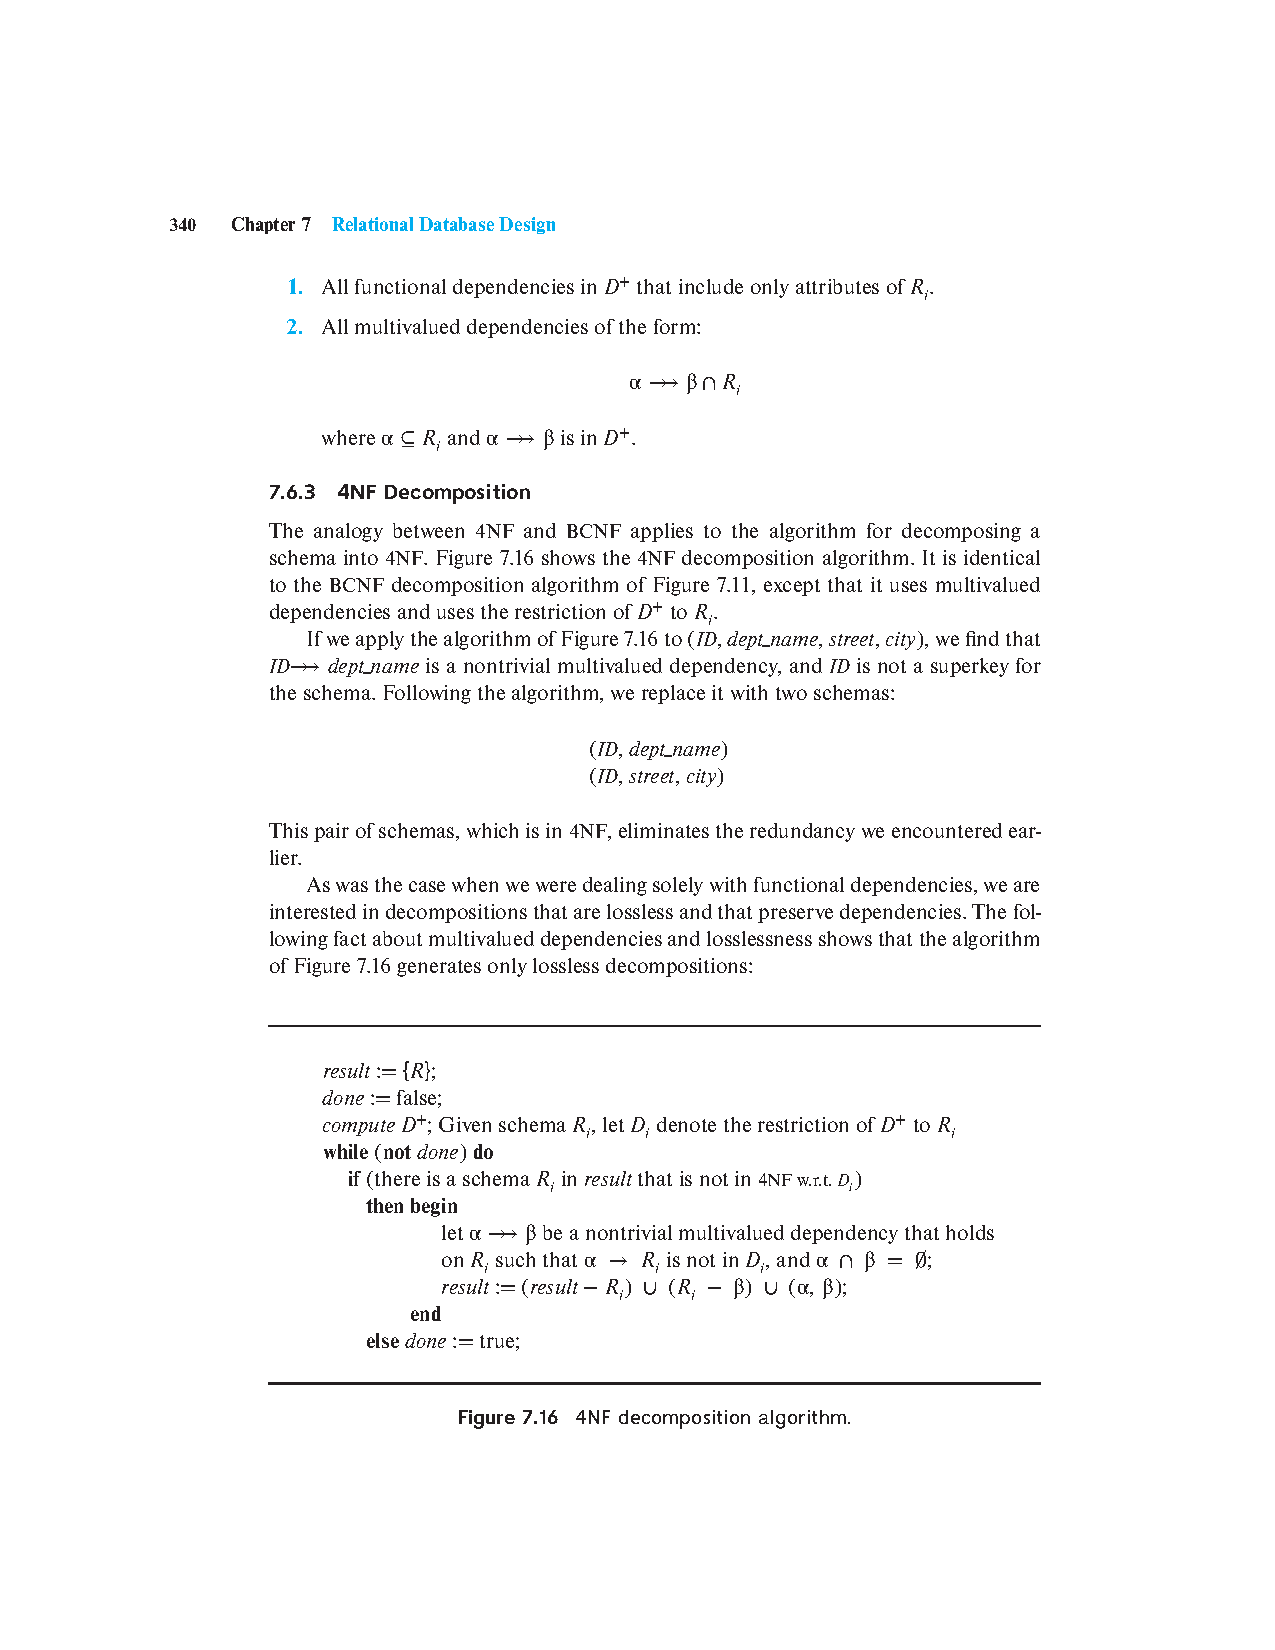
\includegraphics[width=\textwidth, trim={4.5cm 3.5cm 4cm 16.75cm}, clip]{figures/p340_Decomposition_4NF}
    \end{center}
\end{frame}

\begin{frame}{Example}
    \footnotesize
    \begin{itemize}
        \item $R =(A, B, C, G, H, I)$ \\
            \begin{equation*}
                \begin{align*}
                    F = \{  A  &\twoheadrightarrow B  \\
                            B  &\twoheadrightarrow HI \\
                            CG &\twoheadrightarrow H \}
                \end{align*}
            \end{equation*}

        \item $R$ is not in 4NF since $A \twoheadrightarrow B$ and $A$ is not a superkey for $R$.

        \item Decomposition
            \begin{enumerate}
                \item $R_1 = (A, B)$            \quad [$R_1$ is in 4NF] \pause
                \item $R_2 = (A, C, G, H, I)$   \quad [$R_2$ is not in 4NF, decompose into $R_3$ and $R_4$] \pause
                \item $R_3 = (C, G, H)$         \quad [$R_3$ is in 4NF] \pause
                \item $R_4 = (A, C, G, I)$      \quad [$R_4$ is not in 4NF, decompose into $R_5$ and $R_6$] \pause
                    \begin{itemize}
                        \item $A \twoheadrightarrow B$ and $B \twoheadrightarrow HI$ $\longrightarrow$ $A \twoheadrightarrow HI$, (MVD transitivity),
                        \item and hence $A \twoheadrightarrow I$ (MVD restriction to $R_4$). \pause
                    \end{itemize}
                \item $R_5 = (A, I)$            \quad [$R_5$ is in 4NF] \pause
                \item $R_6 = (A, C, G)$         \quad [$R_6$ is in 4NF]
            \end{enumerate}
    \end{itemize}
\end{frame}

\begin{frame}{Further Normal Forms}
    \begin{itemize}
        \item \textbf{Join dependencies} generalize multivalued dependencies:
            \begin{itemize}
                \item lead to \textbf{project-join normal form (PJNF)} (also called fifth normal form).
            \end{itemize}
        \item A class of even more general constraints, leads to a normal form called \textbf{domain-key normal form (DKNF)}.
        \item Problem with these generalized constraints: are hard to reason with, and no set of sound and complete set of inference rules exists.
        \item Hence rarely used.
    \end{itemize}
\end{frame}

\section{Database-Design Process}

\begin{frame}{Overall Database Design Process}
    We have assumed schema R is given:
        \begin{itemize}
            \item $R$ could have been generated when converting E-R diagram to a set of tables.
            \item $R$ could have been a single relation containing \textit{all} attributes that are of interest (called \textbf{universal relation}).
            \item Normalization breaks $R$ into smaller relations.
            \item $R$ could have been the result of some ad hoc design of relations, which we then test/convert to normal form.
        \end{itemize}
\end{frame}

\begin{frame}{E-R Model and Normalization}
    \begin{itemize}
        \item When an E-R diagram is carefully designed, identifying all entities correctly, the tables generated from the E-R diagram should not need further normalization.
        \item However, in a real (imperfect) design, there can be functional dependencies from non-key attributes of an entity to other attributes of the entity:
            \begin{itemize}
                \item Example: an \texttt{employee} entity with:
                    \begin{itemize}
                        \item attributes: \\
                            \quad $department\_name$ and $building$,
                        \item functional dependency: \\
                            \quad $department\_name \rightarrow building$,
                        \item Good design would have made department an entity
                    \end{itemize}

            \end{itemize}
        \item Functional dependencies from non-key attributes of a relationship set possible, but rare (most relationships are binary).
    \end{itemize}
\end{frame}

\begin{frame}{Denormalization for Performance}
    \begin{itemize}
        \item May want to use non-normalized schema for performance
        \item For example, displaying \texttt{prereqs} along with $course\_id$, and $title$ requires join of \texttt{course} with \texttt{prereq},
        \item Alternative 1: Use denormalized relation containing attributes of \texttt{course} as well as \texttt{prereq} with all above attributes...
            \begin{itemize}
                \item faster lookup,
                \item extra space and extra execution time for updates,
                \item extra coding work for programmer and possibility of error in extra code.
            \end{itemize}
        \item Alternative 2: use a materialized view defined as:
            $$
                course \Join prereq
            $$
            \vspace{-5mm}
            \begin{itemize}
                \item Benefits and drawbacks same as above, except no extra coding work for programmer and avoids possible errors.
            \end{itemize}
    \end{itemize}
\end{frame}

\begin{frame}[fragile]{Other Design Issues}
    \begin{itemize}
        \item Some aspects of database design are not caught by normalization.
        \item Examples of bad database design, to be avoided:\\
            Instead of \verb|earnings(company_id, year, amount)|, use
            \begin{itemize}
                \item \verb|earnings_2004|, \verb|earnings_2005|, \verb|earnings_2006|, etc., all on the schema \verb|(company_id, earnings)|.
                    \begin{itemize}
                        \item Above are in BCNF, but make querying across years difficult and needs new table each year.
                    \end{itemize}
                \item
                    \begin{verbatim}
company_year (company_id, earnings_2004,
    earnings_2005, earnings_2006)
                    \end{verbatim}
                    \vspace{-3mm}

                    \begin{itemize}
                        \item Also in BCNF, but also makes querying across years difficult and requires new attribute each year.
                        \item Is an example of a crosstab, where values for one attribute become column names.
                        \item Used in spreadsheets, and in data analysis tools
                    \end{itemize}
            \end{itemize}
    \end{itemize}
\end{frame}

\section{Modeling Temporal Data}

\begin{frame}{Modeling Temporal Data}
    \footnotesize
    \begin{itemize}
        \item \textbf{Temporal data} have an association time interval during which the data are \textit{valid}.
        \item A \textbf{snapshot} is the value of the data at a particular point in time.
        \item Several proposals to extend E-R model by adding valid time to:
            \begin{itemize}
                \footnotesize
                \item attributes, e.g., address of an instructor at different points in time.
                \item entities, e.g., time duration when a student entity exists.
                \item relationships, e.g., time during which an instructor was associated with a student as an advisor.
            \end{itemize}
        \item But no accepted standard...
        \item Adding a temporal component results in functional dependencies like:
            $$
                ID \rightarrow street, city
            $$
            not holding, because the address varies over time.
        \item A temporal functional dependency $X \rightarrow Y$ holds on schema $R$ if the functional dependency $X \longrightarrow Y$ holds on \textit{all} snapshots for \textit{all} legal instances $r(R)$.
    \end{itemize}
\end{frame}

\begin{frame}{Modeling Temporal Data (Cont.)}
    \begin{itemize}
        \footnotesize
        \item In practice, database designers may add start and end time attributes to relations...
            \begin{itemize}
                \footnotesize
                \item E.g., \\
                        \quad \texttt{course(course\_id, course\_title)} \\
                    is replaced by \\
                        \quad \texttt{course(course\_id, course\_title, start, end)}
                \item Constraint: no two tuples can have overlapping valid times,
                \item Hard to enforce efficiently.
            \end{itemize}
        \item Foreign key references may be to current version of data, or to data at a point in time...
            \begin{itemize}
                \footnotesize
                \item E.g., student transcript should refer to course information at the time the course was taken.
            \end{itemize}
    \end{itemize}
\end{frame}

\section{Atomic Domains and First Normal Form}

\begin{frame}{First Normal Form}
    \begin{itemize}
        \item Domain is \textbf{atomic} if its elements are considered to be indivisible units...
            \begin{itemize}
                \item Examples of non-atomic domains:
                    \begin{itemize}
                        \item Set of names, composite attributes.
                        \item Identification numbers like CS101 that can be broken up into parts.
                    \end{itemize}
            \end{itemize}
        \item A relational schema R is in \textbf{first normal form} if the domains of all attributes of $R$ are atomic.
        \item Non-atomic values complicate storage and encourage redundant (repeated) storage of data.
            \begin{itemize}
                \item Example: Set of accounts stored with each customer, and set of owners stored with each account.
                \item We assume all relations are in first normal form (and revisit this in Chapter 22: Object Based Databases).
            \end{itemize}
    \end{itemize}
\end{frame}

\begin{frame}{First Normal Form (Cont.)}
    Atomicity is actually a property of how the elements of the domain are used.
        \begin{itemize}
            \item Example: Strings would normally be considered indivisible.
            \item Suppose that students are given roll numbers which are strings of the form CS0012 or EE1127.
            \item If the first two characters are extracted to find the department, the domain of roll numbers is not atomic.
            \item Doing so is a bad idea: leads to encoding of information in application program rather than in the database.
        \end{itemize}
\end{frame}

% \begin{frame}[fragile]{}
%     \begin{minted}
%     [tabsize=4, obeytabs, frame=lines, framesep=2mm, baselinestretch=1.2, bgcolor=LightGray, fontsize=\scriptsize]{sql}
%     \end{minted}
% \end{frame}

\begin{frame}{}
     \centering
     \Huge End of Chapter 7.
\end{frame}

\section*{Takeaways}

% Tim Duncan's Top 5 Fundamental Takeaways of the Today's Class
\begin{frame}{TDT5FTOTTC}
    \centering
    
\includegraphics[width=0.75\textwidth]{figures/tim.png}
\end{frame}

\begin{frame}{Top 5 Fundamental Takeaways}
    \small
    \begin{enumerate} \pause
        \item[5] Good relational design reduces redundancy and avoids update anomalies by ensuring data is stored without unnecessary repetition or nulls. \pause

        \item[4] Lossless and dependency-preserving decomposition ensures that a schema can be split without losing data or making constraint enforcement inefficient. \pause

        \item[3] Functional dependencies and normal forms guide how to structure schemas to eliminate redundancy while preserving meaningful data relationships. \pause

        \item[2] Canonical covers provide a minimal, simplified set of functional dependencies that retain the original semantics for efficient constraint checking. \pause

        \item[1] Fourth Normal Form (4NF) extends normalization to eliminate redundancy caused by multivalued dependencies, ensuring cleaner data representation.
    \end{enumerate}
\end{frame}

\begin{frame}{Database System Concepts}
    \centering
    
\includegraphics[width=0.5\textwidth]{figures/book_cover.jpg} \\
    \vspace{5mm}
    {
        \tiny
        Content has been extracted from \textit{Database System Concepts}, Seventh Edition, by Silberschatz, Korth and Sudarshan. Mc Graw Hill Education. 2019.\\
        Visit \url{https://db-book.com/}.\\
    }
\end{frame}

\end{document}
